\newpage
\section{Обслуживание пациентов}
\ifthenelse{\isnamedefined{fullversion} \OR \isnamedefined{regversion}}
{
\subsection{Обслуживание пациентов в регистратуре}
\subsubsection {Регистрация обращений} \label{pol_obr}

Каждый раз при обращении пациента в ЛПУ за амбулаторной помощью, в картотеке пациентов для него регистрируется новое обращение. Обращение содержит цель, установленные диагнозы пациента, результаты осмотров и обследований, информацию о назначенных мероприятиях и их выполнении, результат обращения. На основании обращения можно распечатать <<Талон амбулаторного пациента>> (Ф. 025\slash У-12).

Для регистрации обращения на основе предварительной записи следует найти данные пациента в БД (см. п. \ref{cl_find}) и щелкнуть по соответствующей записи левой кнопкой мыши. В появившемся всплывающем окне (Рисунок \ref{img_cl_contrwin}) нужно нажать кнопку 
\includegraphics[scale=0.6]{addg}, справа от соответствующей записи на вкладке \dm{Предварительная запись}. Будет открыта страница \dm{Создание обращения}.

Кнопки \btn{Создать обращение} или 
\includegraphics[scale=0.6]{addb} позволяют создавать обращение без предварительной записи. Кнопки доступны:
\begin{itemize}
 \item Из высплывающего окна картотеки пациентов (Рисунок \ref{img_cl_contrwin});
 \item Со страницы создания и редактирования регистрационной карточки пациента. 
\end{itemize}

Дле регистрации обращения без предварительной записи нужно нажать кнопку \btn{Создать обращение} или кнопку 
\includegraphics[scale=0.6]{addb}. Если на момент регистрации обращения у пациента имеются действующие предварительные записи к другим специалистам, то появится предупреждение во всплывающем окне <<У пациента есть предварительные записи>>.Необходимо убедиться, что предварительные записи были зарегистрированы к другому врачу и только после этого продолжить регистрацию текущего обращения нажатием кнопки \btn{Все равно продолжить}. Отменить создание обращения без предварительной записи можно, нажав кнопку  \btn{Отмена} во всплывающем окне.

После подтверждения будет открыта страница \dm{Создание обращения}. На этой странице, прежде всего, необходимо убедиться, что обращение создано для нужного пациента, проверив его данные в правой верхней части окна. После этого нужно заполнить пустые и изменить неверно заполненные поля в блоке \dm{Основная информация}. Часть полей может быть заполнена на основе данных предварительной записи (если обращение создавалось на основе нее) или значениями по умолчанию.

\begin{vnim}
 Поля \dm{Дата выполнения} и \dm{Время выполнения} на данном этапе заполнять не нужно!
\end{vnim}

Все поля, кроме полей \dm{Дата выполнения} и \dm{Время выполнения} являются обязательными для заполнения.
\begin{itemize}
 \item \dm{Тип обращения} выбирается из списка значение <<Поликлиника>>.
 \item \dm{Источник финансирования} – канал оплаты обращения, выбирается из списка.
 \item \dm{Договор} – номер договора об оплате выбирается из списка. Состав списка зависит от выбранного источника финансирования.
 \item \dm{Тип события} – выбирается из списка. Состав списка изменяется в зависимости от выбранного типа обращения и источника финансирования.
 \item \dm{Лечащий врач} – врач, к которому направляется пациент в поликлинике.
 \item \dm{Подразделение} – отделение поликлиники, куда направляется пациент.
 \item \dm{Дата начала} – по умолчанию устанавливается дата предварительной записи либо текущая дата. При необходимости дату можно изменить.
 \item \dm{Время начала} – по умолчанию устанавливается время предварительной записи либо текущее время. При необходимости время можно изменить.
 \item \dm{Дата выполнения} – дата завершения обслуживания по данному обращению. Должна заполняться врачом.
 \item \dm{Время выполнения} – время закрытия обращения. Должно заполняться врачом.
\end{itemize}

После того как все поля заполнены верно, нужно нажать кнопку \btn{Создать} в правом нижнем углу страницы. Будет осуществлен переход к следующему этапу оформления обращения. Как правило, работа регистратуры ограничивается первым этапом. Последующее заполнение обращения выполняется врачом.

Если была предпринята попытка создания обращения не для того пациента или создание обращения вообще не требуется, следует нажать кнопку \btn{Отменить}. Обращение создано не будет.

\paragraph{Регистрация платных обращений}

Если в качестве источника финансирования обращения выбрано <<Платные услуги>>, то необходимо на странице обращения зарегистрировать данные о плательщике (Рисунок \ref{img_pol_payer}). Рекомендуется сделать это при создании обращения. Однако, можно ввести эти данные и позднее, открыв обращение на редактирование. 

\begin{figure}[ht]\centering
	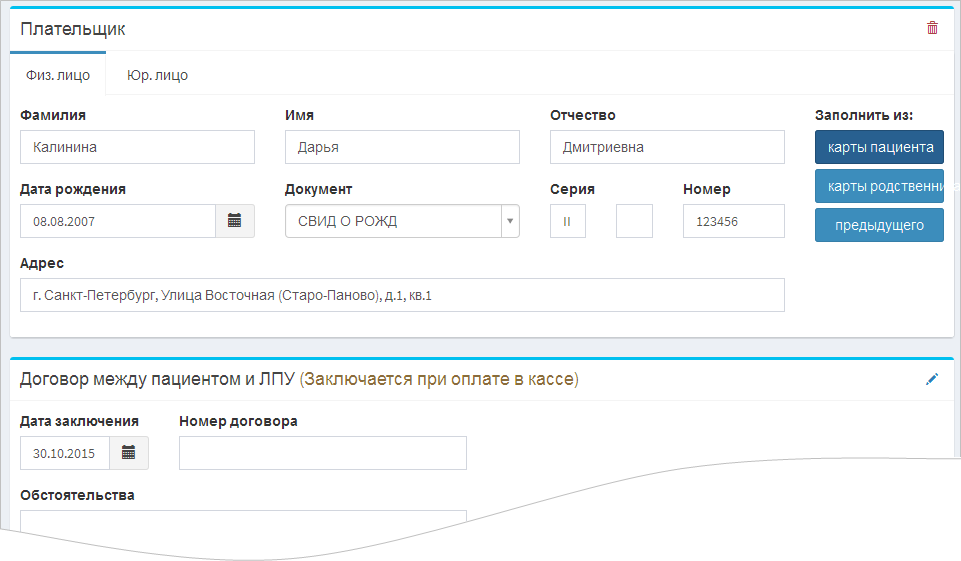
\includegraphics[width = 1\textwidth ,keepaspectratio]{pol_payer}
	\caption{Данные плательщика в обращении}
	\label{img_pol_payer}
\end{figure}

В качестве плательщика может выступать физическое или юридическое лицо.

Если плательщиком является физическое лицо, то необходимо заполнить следующие поля в подразделе \dm{Плательщик} на вкладке \dm{Физ.лицо}:
\begin{itemize}
	\item \dm{Фамилия} -- фамилия плательщика;
	\item \dm{Имя} -- имя плательщика;
	\item \dm{Отчество} -- отчество плательщика;
	\item \dm{Дата рождения} -- дата рождения плательщика;
	\item \dm{Документ} -- тип документа, удостоверяющего личность плательщика. Выбирается из раскрывающегося списка;
	\item \dm{Серия} -- серия документа, удостоверяющего личность плательщика. Серия может быть разбита на 2 отдельных поля;
	\item \dm{Номер} -- номер документа, удостоверяющего личность плательщика. 
	\item \dm{Серия} -- серия документа, удостоверяющего личность плательщика;
	\item \dm{Адрес} -- адрес регистрации плательщика, записывается в виде текстовой строки. 
\end{itemize}

Кнопки, расположенные справа от полей подраздела \dm{Плательщик}, позволяют в некоторых случаях автоматизировать заполнение данных полей. 
\begin{itemize}
	\item Кнопка \btn{карты пациента} позволяет скопировать в поля подраздела \dm{Плательщик} на вкладке \dm{Физ.лицо} данные пациента. Данную кнопку можно применять, если сам пациент является плательщиком.
	\item Кнопка \btn{карты родственника} позволяет скопировать в поля подраздела \dm{Плательщик} на вкладке \dm{Физ.лицо} данные одного из родственников пациента. При нажатии на данную кнопку появляется всплывающее окно, где необходимо выбрать одного из родственноков пациента и нажать кнопку \btn{Выбрать}. Для использования данного способа необходимо, чтобы родственник пациента был зарегистрирован в разделе \dm{Связи} регистрационной карточки текущего пациента.
	\item Кнопка \dm{предыдущего} позволяет скопировать данные плательщика из предыдущего обращения пациента (если такое имеется).
\end{itemize} 

Если плательщиком является юридическое лицо, то необходимо перейти на вкладку \dm{Юр.лицо} в подразделе \dm{Плательщик} и выбрать название организации-плательщика из раскрывающегося списка. Вверху списка предусмотрено поле поиска организации. Список организаций фильтруется в соответствии с текстом, введенным в поле поиска. Все необходимые реквизиты организации-плательщика должны быть заполнены в справочнике организаций и не требуют повторного заполнения.

\paragraph{Регистрация услуг} \label{ev_regusl}

В случае обращения пациента за медицинскими услугами на платной основе, необходимо зарегистрировать список услуг, которые будут оказаны пациенту, согласовать стоимость и оформить договор на оказание соответствующих услуг.

Регистрация услуг выполняется на странице редактирования обращения (Рисунок \ref{img_pol_usl}). Необходимо ввести часть наименования услуги в поле поиска, после чего выбрать нужную запись или несколько записей, появившихся в списке ниже, щелкнув по ним левой кнопкой мыши. Выбранные строки появятся в списке \dm{Выбранные услуги}.

\begin{figure}[ht]\centering
	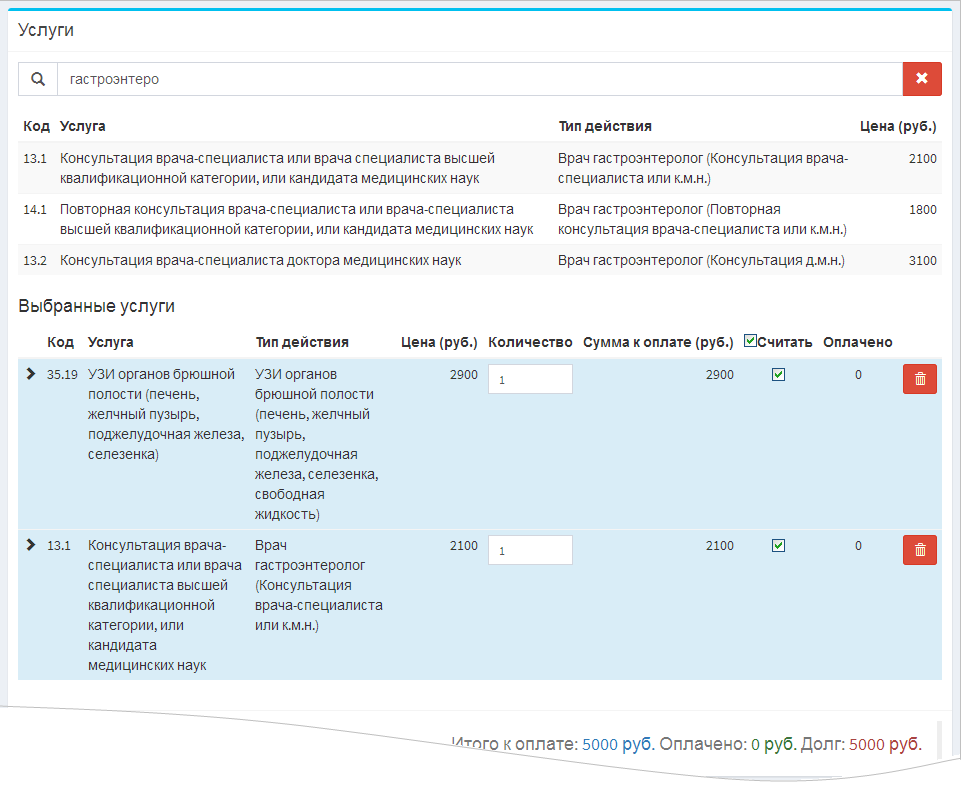
\includegraphics[width = 1\textwidth ,keepaspectratio]{pol_usl}
	\caption{Регистрация услуг в обращении}
	\label{img_pol_usl}
\end{figure}

Для выбранных услуг можно изменить количество в ячейке \dm{Количество} и установить флажок \dm{Считать} для включения стоимость услуг в итоговую сумму в строке <<Итого к оплате>> под таблицей. 

После регистрации требуемого набора услуг необходимо сохранить обращение, после чего распечатать договор и другие платежные документы, нажав кнопку 
\includegraphics[scale=0.6]{print}, выбрав соответствующие пункты из списка и нажав кнопку \btn{Печать}.
}{}

\ifthenelse{\NOT \isnamedefined{regversion}}{

\subsection{Обслуживание пациентов врачом} \label{pol_doc}
\subsubsection{Прием пациентов} \label{pol_doc_priem}

Если в ЛПУ ведется предварительная запись пациентов на прием по расписанию, то обслуживание пациентов врачом выполняется из раздела \dm{Прием пациентов}. Раздел будет доступен только при наличии у пользователя прав на выполнение данной функции.
Для перехода к обслуживанию пациентов следует на панели управления в верхней части страницы нажать кнопку \dm{Прием пациентов}. Откроется страница управления приемом пациентов (Рисунок \ref{img_ev_obsl}). 

\begin{figure}[ht]\centering
	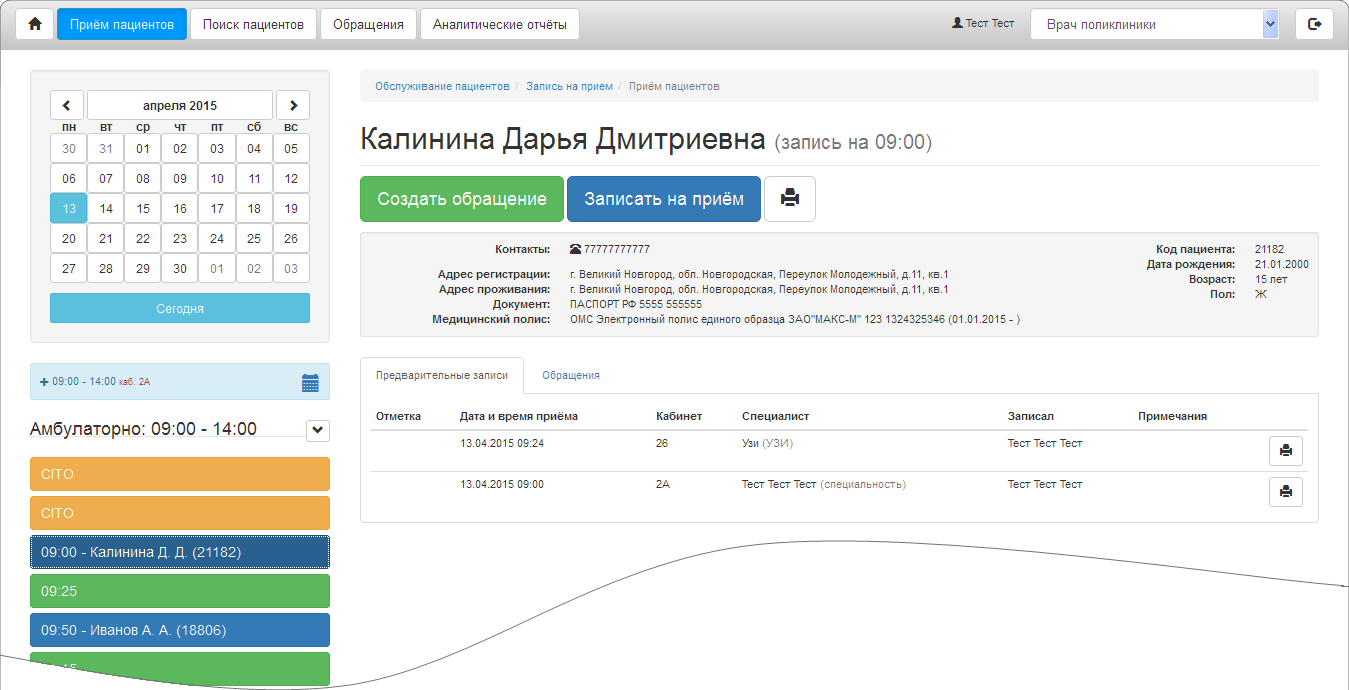
\includegraphics[width = 1\textwidth ,keepaspectratio]{ev_obsl}
	\caption{Страница приема пациентов}
	\label{img_ev_obsl}
\end{figure}

\ifthenelse{\NOT \isnamedefined{doctorversion}}
{
Внешний вид страницы приема пациентов для врача диагностики отличается наличием в левом верхнем углу раскрывающегося списка выбора диагностического кабинета (Рисунок \ref{img_ev_obsldiag}). Это связано с тем, что для диагностических исследований запись ведется не к конкретному врачу, а в определенный кабинет.

\begin{figure}[ht]\centering
	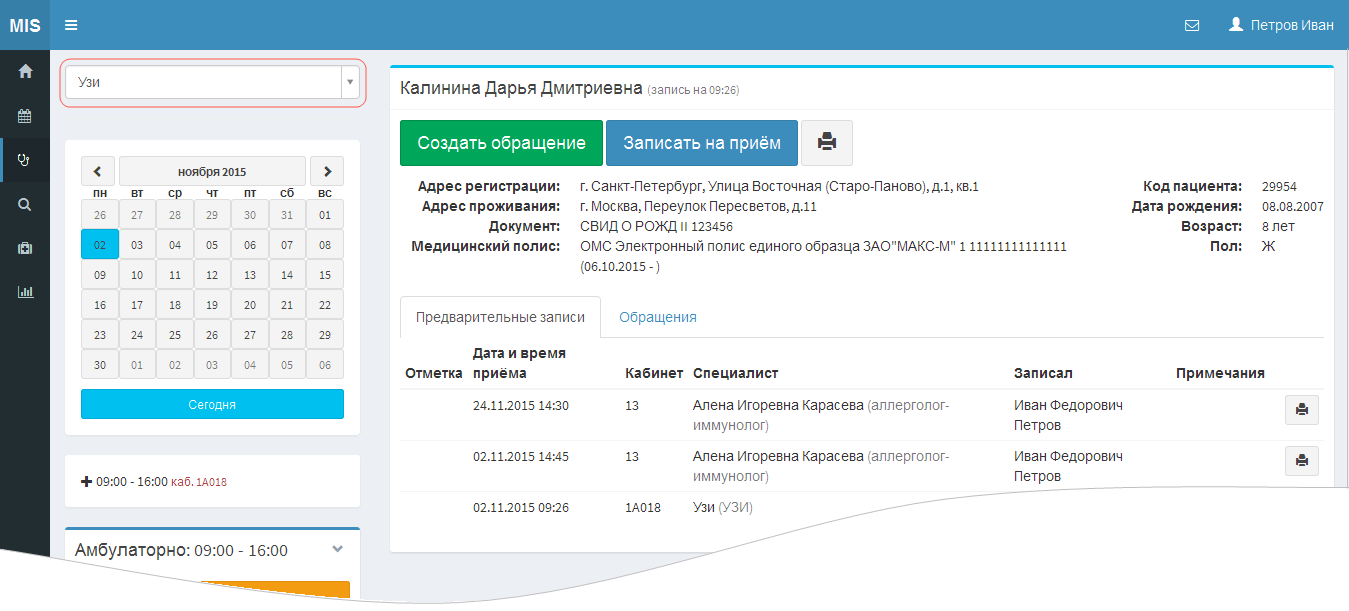
\includegraphics[width = 0.8\textwidth ,keepaspectratio]{ev_obsldiag}
	\caption{Отличие страницы приема пациентов врача диагностики}
	\label{img_ev_obsldiag}
\end{figure}
}{}

Страница приема пациентов разделена на две части: в левой части расположена панель выбора пациента и просмотра текущих записей, в правой части -- область отображения данных выбранного пациента и выполнения основных операций по его обслуживанию.

На панели, расположенной в левой части страницы отображается расписание \ifthenelse{\NOT \isnamedefined{diagnversion}}{~текущего пользователя (под именем которого был осуществлен вход в систему)}{} \ifthenelse{\isnamedefined{fullversion} \OR \isnamedefined{assistversion}}{(для врача поликлиники) или }{} \ifthenelse{\NOT \isnamedefined{doctorversion}}{~выбранного   кабинета}{} \ifthenelse{\isnamedefined{fullversion} \OR \isnamedefined{assistversion}}{(для врача диагностики)}{}. В верхней части панели находится календарь, с помощью которого можно выбрать день для обслуживания или записи пациентов (работа с календарем подробно описана в разделе \ref{gen_cal}). После выбора дня в календаре, в нижней части страницы появляется расписание работы врача \ifthenelse{\NOT \isnamedefined{diagnversion}}{(кабинета)}{} на этот день. По умолчанию, расписание прошлых периодов скрывается. Для того чтобы раскрыть его, нужно нажать кнопку \includegraphics[scale=0.6]{rollup}.    
\ifthenelse{\isnamedefined{fullversion} \OR \isnamedefined{assistversion} \OR \isnamedefined{diagnversion}}{Для врача диагностики перед выбором дня в календаре нужно выбрать кабинет, в котором осуществляется прием.}{} 

Непосредственно под календарем расположены данные расписания выбранного дня: часы приема и номер кабинета. Нажав на кнопку 
\includegraphics[scale=0.6]{ttbl}, можно просмотреть \ifthenelse{\isnamedefined{fullversion} \OR \isnamedefined{assistversion} \OR \isnamedefined{doctorversion}}{все свое расписание}{} \ifthenelse{\isnamedefined{fullversion} \OR \isnamedefined{assistversion}}{\slash}{} \ifthenelse{\isnamedefined{fullversion} \OR \isnamedefined{assistversion} \OR \isnamedefined{doctorversion}}{расписание выбранного кабинета}{}~на отдельной странице.

В левой нижней части страницы расположен список интервалов записи на прием. Интервалы могут иметь следующие цвета:
\begin{itemize}
	\item \dm{Зеленый} -- свободный интервал, на который можно записать пациента.
	\item \dm{Синий} -- интервал, на который записан пациент. Фамилия пациента указана в заголовке интервала.
	\item \dm{Оранжевый} интервал с надписью \dm{<<CITO>>} -- интервал для записи экстренных пациентов;
	\item \dm{Серый} интервал с надпиью \dm{Сверх плана} -- интервал для записи пациентов сверх плана;
	\item \dm{Бледно-зеленый}, \dm{бледно-оранжевый} и \dm{бледно-серый} -- интервалы за прошедший период времени. Запись пациента на этот период невозможна. 
\end{itemize}

При нажатии на интевал синего цвета, в правой части страницы появляется информация о пациенте, который записан на данное время:
\begin{itemize}
	\item В левом верхнем углу расположена кнопка \btn{Создать обращение} (если по выбранной предварительной записи еще не было создано обращение) или \btn{Открыть обращение ...} (если оно уже создано).
	\item Рядом расположена кнопка \btn{Записать на прием}, при нажатии на которую открывается страница предварительной записи пациента к другим специалистам (раздел \ref{pol_predvz})
	\item Кнопка 
\includegraphics[scale=0.6]{print}, расположенная в верхней части страницы, позволяет распечатать маршрутный лист пациента.
	\item Под кнопками располагается секция, содержащая основные сведения о пациенте: ФИО, возраст, код пациента, контактные данные, адреса, данные документов.
	\item В нижней части страницы отображаются данные о предварительных записях и обращениях пациента. Данные о предварительных записях доступны на вкладке  \dm{Предварительные записи}. Нажатием на кнопку 
\includegraphics[scale=0.6]{print} напротив соответствующей предварительной записи можно распечатать маршрутный лист и другие документы по данной предварительной записи. Если обращение по предварительной записи уже создано, то его так же можно открыть, щелкнув по кнопке 
\includegraphics[scale=0.6]{goto} соответствующей строки в списке предварительной записи. Для просмотра данных обо всех  обращениях пациента необходимо перейти на вкладку \dm{Обращения}. Щелкнув левой кнопкой мыши по записи об обращении, можно открыть карточку обращения для просмотра или редактирования.
\end{itemize}  

\paragraph{Последовательность действий при регистрации приема пациента}

При обращении пациента по предварительной записи, порядок действий врача должен быть следующим:
\begin{enumerate}
	\item В верхней части страницы на панели управления нажать кнопку \btn{Прием пациентов}.
	\ifthenelse{\NOT \isnamedefined{doctorversion}}{\item В левом верхнем углу открывшейся страницы выбрать нужный диагностический кабинет 	\ifthenelse{\NOT \isnamedefined{diagnversion}}{(для врача диагностики)}{}.}{} 
	\item По умолчанию открывается список предварительной записи на текущую дату. При необходимости, изменить дату, выбрав ее в календаре (см. раздел \ref{gen_cal}) в левой верхней части страницы.
	\item Щелкнуть левой кнопкой мыши по фамилии пациента в списке предварительной записи. В правой части страницы появятся данные о выбранном пациенте.
	\item Нажать кнопку \btn{Создать обращение} или \btn{Открыть обращение ....} в левом верхнем углу основной части страницы. Откроется страница обращения пациента.
	\item Заполнить и сохранить данные текущего обращения пациента (раздел \ref{ev_obr})
	\item Вернуться на страницу \dm{Прием пациентов} и перейти к обслуживанию следующего пациента.
\end{enumerate}

\paragraph{Запись пациента на повторный прием} 

Запись пациента на повторный прием удобно выполнять на странице \dm{Прием пациентов}. Для этого нужно:
\begin{enumerate}
	\item Найти пациента в списке предварительной записи и щелкнуть по нему левой кнопкой мыши. Данные пациента появятся в правой части страницы. Если непосредственно перед этим выполнялось обслуживание пациента, то данное действие уже выполнено.
	\item В календаре в левой верхней части страницы выбрать дату, на которую следует записать пациента на повторный прием. В левой нижней части страницы появится список интервалов записи на выбранный день.
	\item Щелкнуть левой кнопкой мыши по любому из свободных интервалов.
	\item В появившемся диалоговом окне выбрать тип записи из раскрывающегося списка и подтвердить запись пациента, нажав кнопку \btn{Записать}. Интервал окрасится в синий цвет и в его названии появится фамилия пациента.
\end{enumerate} 

\paragraph{Запись пациента к другим специалистам}

Со страницы \dm{Прием пациентов} можно так же записать пациента к другим специалистам. Для этого нужно щелкнуть левой кнопкой мыши по фамилии пациента в списке предварительной записи и после того, как данные пациента появятся в правой части страницы, нажать кнопку \btn{Записать на прием} в правой верхней части страницы. В результате, откроется страница предварительной записи на прием пациента к другим специалистам (Рисунок \ref{img_pol_ttblview}). Работа с этой страницей подробно описана в разделе \ref{pol_predvz}

\subsubsection{Работа с обращениями}
\paragraph{Регистрация обращений}

При создании обращения со страницы \dm{Прием пациентов} открывается страница \dm{Создание обращения} (Рисунок \ref{img_ev_obrnew}). Часть полей заполнена на основе  предварительной записи либо значениями по умолчанию. 

\begin{figure}[ht]\centering
	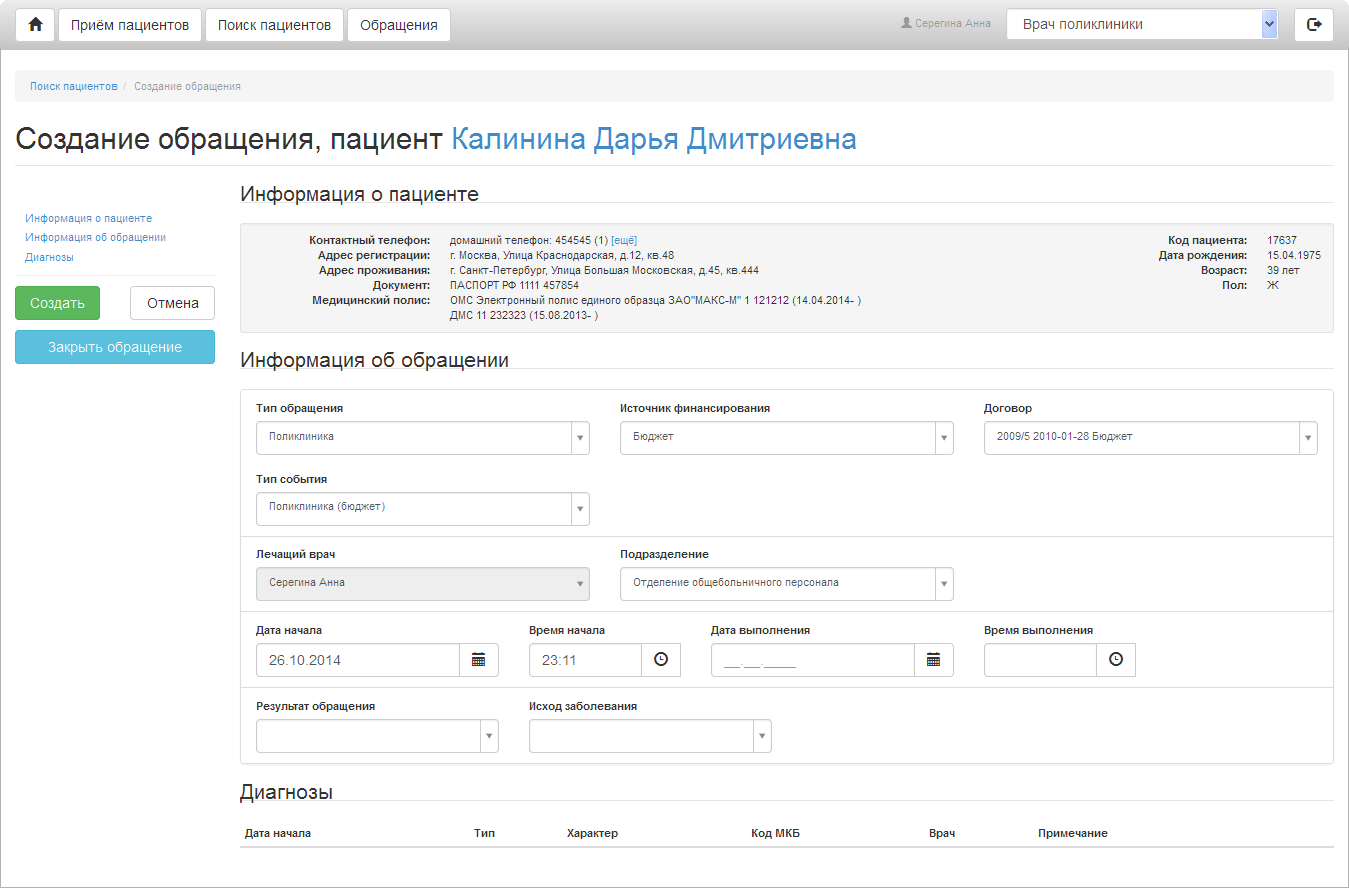
\includegraphics[width = 1\textwidth ,keepaspectratio]{ev_obrnew}
	\caption{Создание обращения}
	\label{img_ev_obrnew}
\end{figure}

При регистрации обращения следует проверить и при необходимости скорректировать следующие данные:
\begin{itemize}
	\item \dm{Тип обращения} выбирается из списка значение <<Поликлиника>> для амбулаторных и <<Диагностика>> для диагностических обращений. Поле обязательно для заполнения.
	\item \dm{Источник финансирования} – канал оплаты обращения, выбирается из списка. По умолчанию устанавливается первый доступный для пациента источник финансирования. При регистрации обращения нужно обратить особое внимание на правильность заполнения данного поля. Поле обязательно для заполнения.
	\item \dm{Договор} –- номер договора об оплате выбирается из списка. Состав списка договоров зависит от выбранного типа обращения и источника финансирования, и составляется индивидуально для каждого пациента. Если в списке доступных договоров присутствует только одна запись, то этот договор устанавливается в поле автоматически. Поле обязательно для заполнения.
	\item \dm{Тип события} -– выбирается из списка. Состав списка изменяется в зависимости от выбранного типа обращения и источника финансирования. Если в отобранном списке присутствует только одна запись, то она устанавливается в поле автоматически. Поле обязательно для заполнения.
	\item \dm{Лечащий врач} –- в поле должна быть указана фамилия врача, создавшего обращение. Поле заполняется только для обращений типа <<Поликлиника>>. По умолчанию указывается фамилия текущего пользователя. Лечащий врач выбирается из раскрывающегося списка. Для поиска в списке следует ввести часть фамилии врача или фамилию полностью, а затем выбрать из предложенных вариантов.
	\item \dm{Подразделение} –- отделение поликлиники, в котором обслуживается пациент. По умолчанию указывается подразделение, к которому относится выбранный лечащий врач. Поле обязательно для заполнения.
	\item \dm{Дата начала} –- по умолчанию устанавливается дата согласно предварительной записи. При необходимости дату можно изменить. Поле обязательно для заполнения.
	\item \dm{Время начала} –- по умолчанию устанавливается время согласно предварительной записи. При необходимости время можно изменить. Поле обязательно для заполнения.
	\item \dm{Дата выполнения} –- дата завершения обслуживания по данному обращению. При регистрации обращения данное поле нужно оставить пустым.
	\item \dm{Время выполнения} -– время закрытия обращения. При регистрации обращения поле нужно оставить пустым.
%	\item \dm{Результат обращения} -- выбирается из списка. При регистрации обращения поле нужно оставить пустым.
%	\item \dm{Исход заболевания} -- выбирается из списка. При регистрации обращения поле нужно оставить пустым.
\end{itemize}

После того как все поля заполнены верно, нужно нажать кнопку \btn{Создать} в левой части страницы. Обращение будет создано с указанными параметрами.  Карточка обращения откроется для редактирования.

\subsection{Карточка обращения} \label{ev_obr}

Карточка обращения состоит из нескольких разделов, которые размещаются последовательно друг за другом. Перемещаться  между разделами можно с помощью колеса прокрутки мыши либо полосы вертикальной прокрутки на странице, а так же с помощью ссылок c названиями разделов в левой части страницы (Рисунок \ref{img_ev_obrcard}). 

\begin{figure}[!ht]\centering
	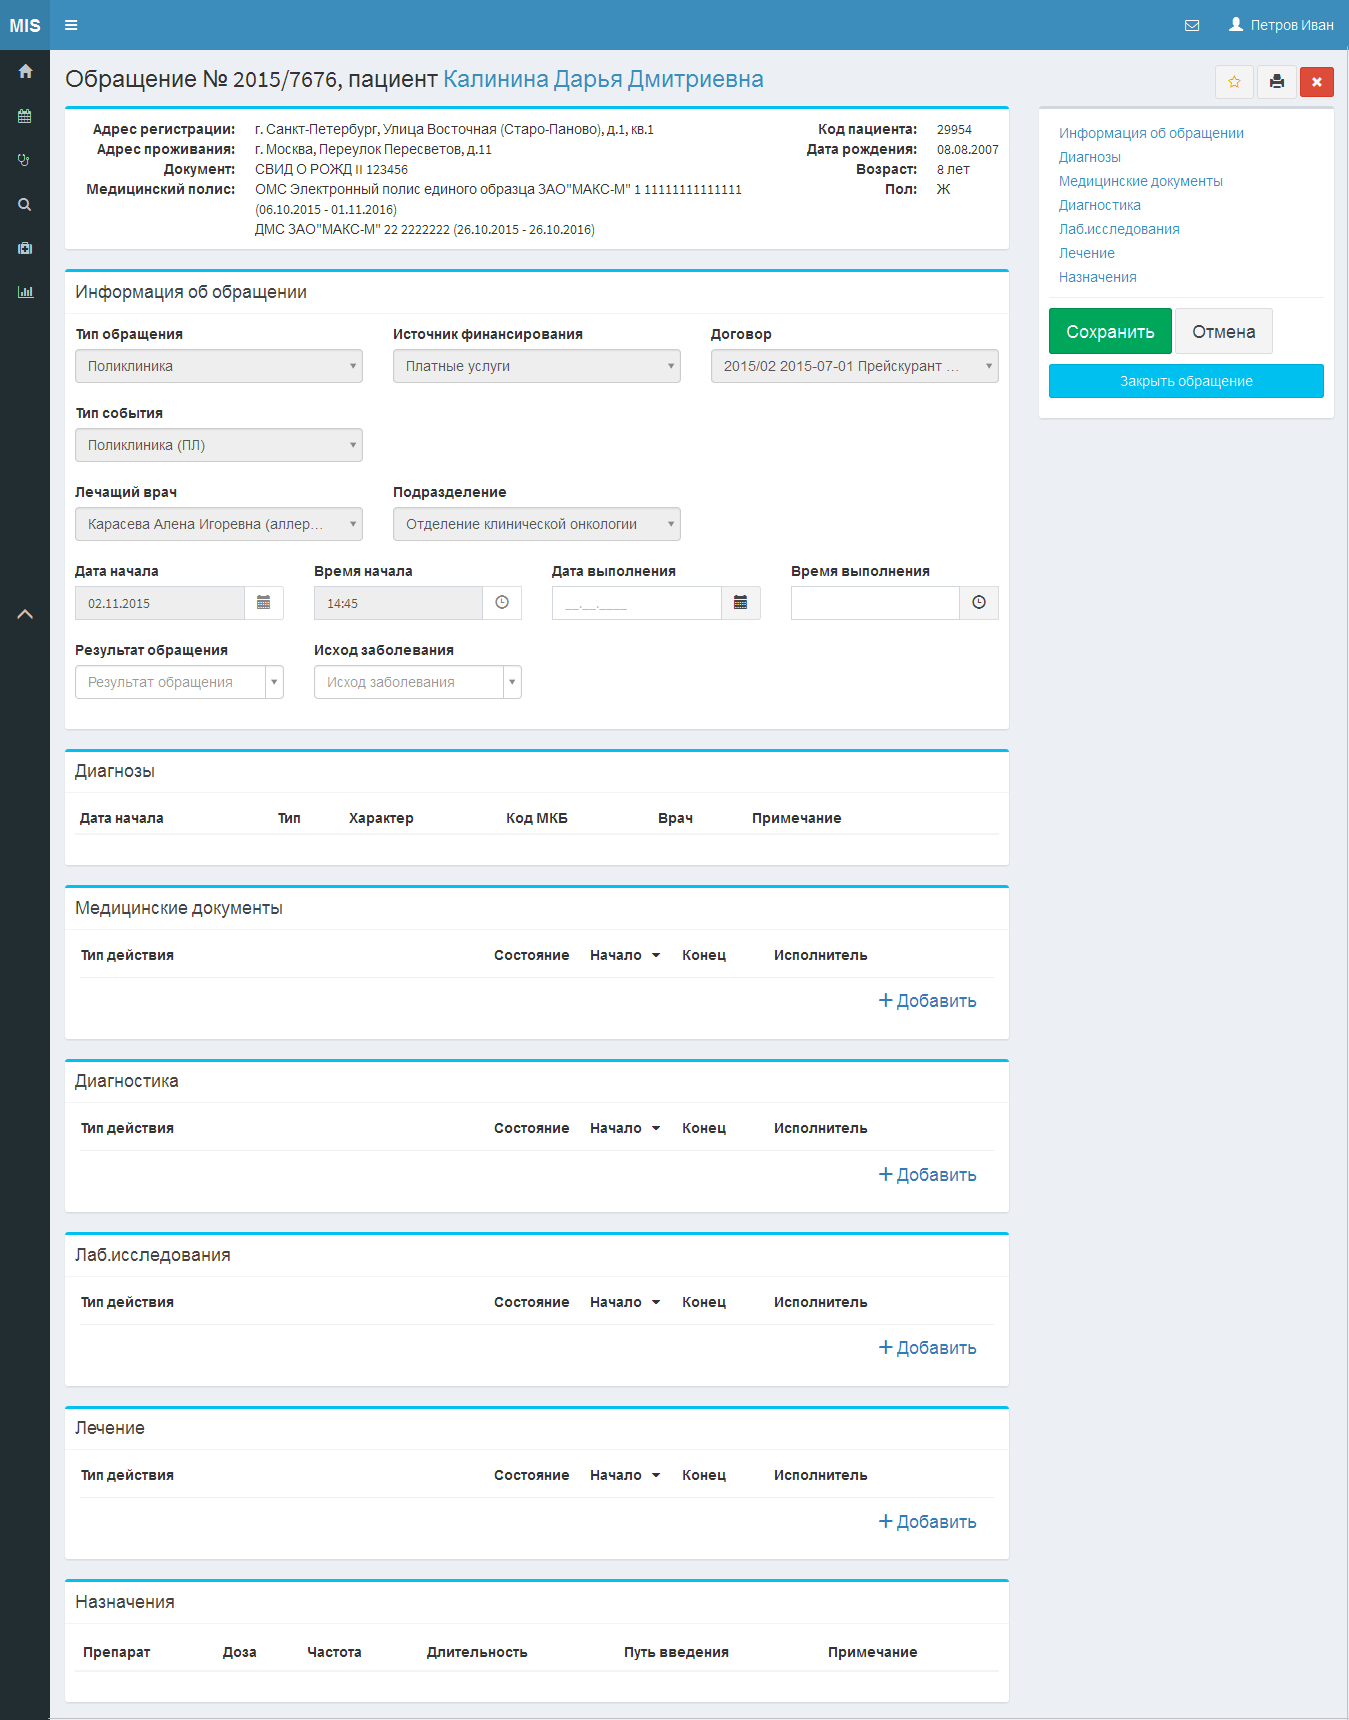
\includegraphics[width = 1\textwidth ,keepaspectratio]{ev_obrcard}
	\caption{Карточка обращения}
	\label{img_ev_obrcard}
\end{figure}

\begin{itemize}
 \item Раздел \dm{Информация о пациенте} содержит краткую информацию о пациенте, для которого создано данное обращение. 
 \item Раздел \dm{Информация об обращении} содержит общие сведения о случае обслуживания, которые учитываются в стат.талоне и других документах. В основном, это поля, которые заполняются при создании обращения. Большинство из них недоступно для редактирования.
 \ifthenelse{\isnamedefined{fullversion}}{\item Раздел \dm{Услуги} содержит перечень услуг предоставленных пациенту, подлежащих оплате по указанному в обращении каналу финансирования;}{}
 \ifthenelse{\isnamedefined{fullversion}}{\item Раздел \dm{Плательщик} доступен только для платных обращений и содержит данные плательщика;}{}
 \item Раздел \dm{Диагнозы} содержит список диагнозов, установленных в рамках данного обращения;
 \ifthenelse{\NOT \isnamedefined{diagnversion}}{\item Раздел \dm{Медицинские документы} содержит направления на консультации и результаты осмотров врача;}{}
 \item Раздел \dm{Диагностика} содержит направления на инструментальные исследования и их результаты;
 \item Раздел \dm{Лаб.исследования} содержит направления на лабораторные исследования и их результаты;
 \ifthenelse{\NOT \isnamedefined{diagnversion}}{\item Раздел \dm{Лечение} содержит направление на медикаментозное, физиотерапевтическое и другие виды лечения и данные о их выполнении.}{}
\end{itemize}
 
В зависимости от роли пользователя в системе и параметров обращения, некоторые разделы могут быть недоступны. Далее каждый из разделов будет рассмотрен более подробно.

\subsubsection{Информация о пациенте}

В верхней части карточки обращения отображается основная информация о пациенте. Данные доступны только для просмотра. Для просмотра расширенной информации о пациенте можно щелкнуть левой кнопкой мыши по фамилии пациента в заголовке страницы. Раскроется карточка пациента, так же доступная только для просмотра. 

\subsubsection{Информация об обращении}

В этом разделе значительная часть данных заполняется на этапе создания обращения и в дальнейшем не подлежит редактированию. Остальные поля (такие как дата выполнения и результат обращения) заполняются при закрытии обращения. 

При создании обращения должны быть заполнены следующие поля (не доступны для редактирования в карточке обращения):
\begin{itemize}
  \item \dm{Тип обращения};
  \item \dm{Источник финансирования};
  \item \dm{Договор};
  \item \dm{Тип события};
  \item \dm{Лечащий врач} (только для типа обращения <<Поликлиника>>);
  \item \dm{Подразделение};
  \item \dm{Дата начала};
  \item \dm{Время начала};
\end{itemize}

Поля, которые необходимо заполнить перед закрытием обращения:
\begin{itemize}   
  \item \dm{Дата выполнения} –- дата завершения обслуживания по данному обращению;
  \item \dm{Время выполнения} -– время закрытия обращения;
  \item \dm{Результат обращения} -- выбирается из списка;
  \ifthenelse{\NOT \isnamedefined{diagnversion}}{\item \dm{Исход заболевания} -- выбирается из списка.}{}
\end{itemize}

\ifthenelse{\isnamedefined{fullversion}}{
\subsubsection{Услуги}

В данном разделе содержится список услуг, предоставленных пациенту в рамках обращения и выставляемых к оплате.
Добавление услуг в список подробно описано в разделе \ref{ev_regusl}

\subsubsection{Плательщик} \label{ev_obr_payer}

Если в качестве источника финансирования обращения выбрано <<Платные услуги>>, то необходимо на странице обращения зарегистрировать данные о плательщике (Рисунок \ref{img_pol_payer}). Как правило, это делается при создании обращения, но, можно ввести эти данные и позднее, открыв обращение на редактирование. 

В данном разделе имеются 2 вкладки: 
\begin{itemize}
 \item \dm{Физ.лицо} -- содержит данные физического лица.
 \item \dm{Юр.лицо} -- содержит ссылку на карточку организации. 
\end{itemize}

При регистрации плательщика должна заполняться только одна из вкладок в зависимости от принадлежности плательщика.

На вкладке \dm{Физ.лицо} необходимо заполнить следующие поля:
\begin{itemize}
	\item \dm{Фамилия} -- фамилия плательщика;
	\item \dm{Имя} -- имя плательщика;
	\item \dm{Отчество} -- отчество плательщика;
	\item \dm{Дата рождения} -- дата рождения плательщика;
	\item \dm{Документ} -- тип документа, удостоверяющего личность плательщика. Выбирается из раскрывающегося списка;
	\item \dm{Серия} -- серия документа, удостоверяющего личность плательщика. Серия может быть разбита на 2 отдельных поля;
	\item \dm{Номер} -- номер документа, удостоверяющего личность плательщика. 
	\item \dm{Серия} -- серия документа, удостоверяющего личность плательщика;
	\item \dm{Адрес} -- адрес регистрации плательщика, записывается в виде текстовой строки. 
\end{itemize}

Кнопки, расположенные справа от полей подраздела \dm{Плательщик}, позволяют в некоторых случаях автоматизировать заполнение данных полей. 
\begin{itemize}
	\item Кнопка \btn{карты пациента} позволяет скопировать в поля подраздела \dm{Плательщик} на вкладке \dm{Физ.лицо} данные пациента. Данную кнопку можно применять, если сам пациент является плательщиком.
	\item Кнопка \btn{карты родственника} позволяет скопировать в поля подраздела \dm{Плательщик} на вкладке \dm{Физ.лицо} данные одного из родственников пациента. При нажатии на данную кнопку появляется всплывающее окно, где необходимо выбрать одного из родственноков пациента и нажать кнопку \btn{Выбрать}. Для использования данного способа необходимо, чтобы родственник пациента был зарегистрирован в разделе \dm{Связи} регистрационной карточки текущего пациента.
	\item Кнопка \dm{предыдущего} позволяет скопировать данные плательщика из предыдущего обращения пациента (если такое имеется).
\end{itemize} 

На вкладке \dm{Юр.лицо} название организации-плательщика выбирается из раскрывающегося списка. Вверху списка предусмотрено поле поиска организации. Список организаций фильтруется в соответствии с текстом, введенным в поле поиска. Все необходимые реквизиты организации-плательщика должны быть заполнены в справочнике организаций и не требуют повторного заполнения.
}{}

\subsubsection{Диагнозы}

Диагнозы, указанные в медицинских записях, входящих в состав данного обращения, автоматически добавляются в данный раздел.

Щелчок левой кнопкой мыши по строке с наименованием диагноза позволяет перейти к просмотру медицинской записи, где был установлен выбранный диагноз. Если документ НЕ завершен, и пользователь имеет достаточно прав для редактирования документа, диагноз можно изменить или удалить внутри медицинскй записи.

\subsubsection{Общие принципы работы с медицинскими записями} \label{pol_obr_gen}

Медицинские записи делятся на следующие типы:
\begin{itemize}
 \item \dm{Медицинские документы} для регистрации результатов осмотров и консультаций врачей-специалистов;
 \item \dm{Диагностика} для регистрации направлений на инструментально-диагностические исследования и их результатов;
 \item \dm{Лаб.исследования} для регистрации направлений на лабораторные исследования и их результатов;
 \item \dm{Лечение} для регистрации направлений на лечебные процедуры, а так же регистрации медикаментозных назначений. 
\end{itemize}

\paragraph{Создание медицинских записей} \label{pol_obr_mdnew}

Для добавления новой медицинской записи следует нажать кнопку \btn{Создать} в конце списка документов требуемого раздела. При этом появляется новое всплывающее окно, содержащее дерево видов медицинских записей (Рисунок \ref{img_ev_obr_addmd}).

\begin{figure}[ht]\centering
 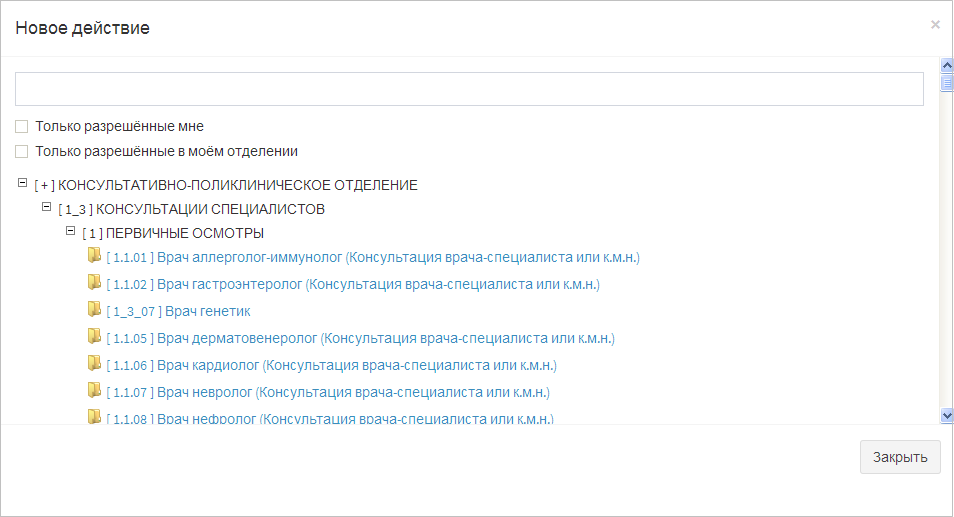
\includegraphics[width = 1\textwidth ,keepaspectratio]{ev_obr_addmd}
 \caption{Создание нового документа}
 \label{img_ev_obr_addmd}
\end{figure}

\begin{vnim}
 Кнопка \btn{Создать} доступна только при наличии у пользователя права на добавление документов соответствующего типа в данное обращение.
\end{vnim} 

В дереве присутствуют группы и виды документов. Виды документов слева помечены значком с изображением раскрытой желтой папки. Их можно выбрать для создания медицинской записи. Группы документов предназначены только для систематизации видов документов и удобства поиска. Они имеют слева знак <<$+$>> (если группа свернута) или <<$-$>> (если группа раскрыта). При нажатии на наименование группы она меняет свое состояние (сворачивается или разворачивается в зависимости от предыдущего состояния). По умолчанию дерево типов документов полностью развернуто. 

В верхней части окна находится поле поиска. При вводе текста в него, осуществляется фильтрация видов документов в дереве -- отображаются только виды, в наименовании которых встречается введенное буквосочетание и группы, содержащие их. Остальные  группы и виды документов скрываются. Фильтрация производится аналогично другим справочникам системы (см. раздел \ref{gen_filtr}). 

%Флажок \dm{Только разрешенные в моем отделении} ограничивает список категорий лишь теми, которые разрешены в отделении к которому прикреплен пользователь. При необходимости можно снять данный флажок тогда список будет содержать все категории документов, доступные для создания данным пользователем.

%Флажок \dm{Только разрешенные мне} ограничивает список категорий лишь теми, которые разрешены текущему пользователю. При необходимости можно снять данный флажок тогда список будет содержать все категории документов, доступные для создания данным пользователем.

\begin{prim}
 Для облегчения поиска список доступных категорий документов для конкретного пользователя (или группы пользователей) может быть ограничен настройками системы. Если в списке отсутствует документ, необходимый для работы, следует обратиться к администратору системы.
\end{prim} 

Для создания документа необходимо щелкнуть левой кнопкой мыши по наименованию соответствующего типа документа, после чего откроется страница редактирования медицинского документа (Рисунок \ref{img_ev_obr_mdedt}). Для различных типов медицинских записей процедура создания может немного отличаться. Особенности быдут рассмотрена в разделах, посвященных отдельным типам медицинских записей.

\paragraph{Редактирование медицинских записей} \label{ev_obr_mdedt}

Любая медицинская запись содержит название документа, учетные данные и основную части.

\begin{figure}[ht]\centering
 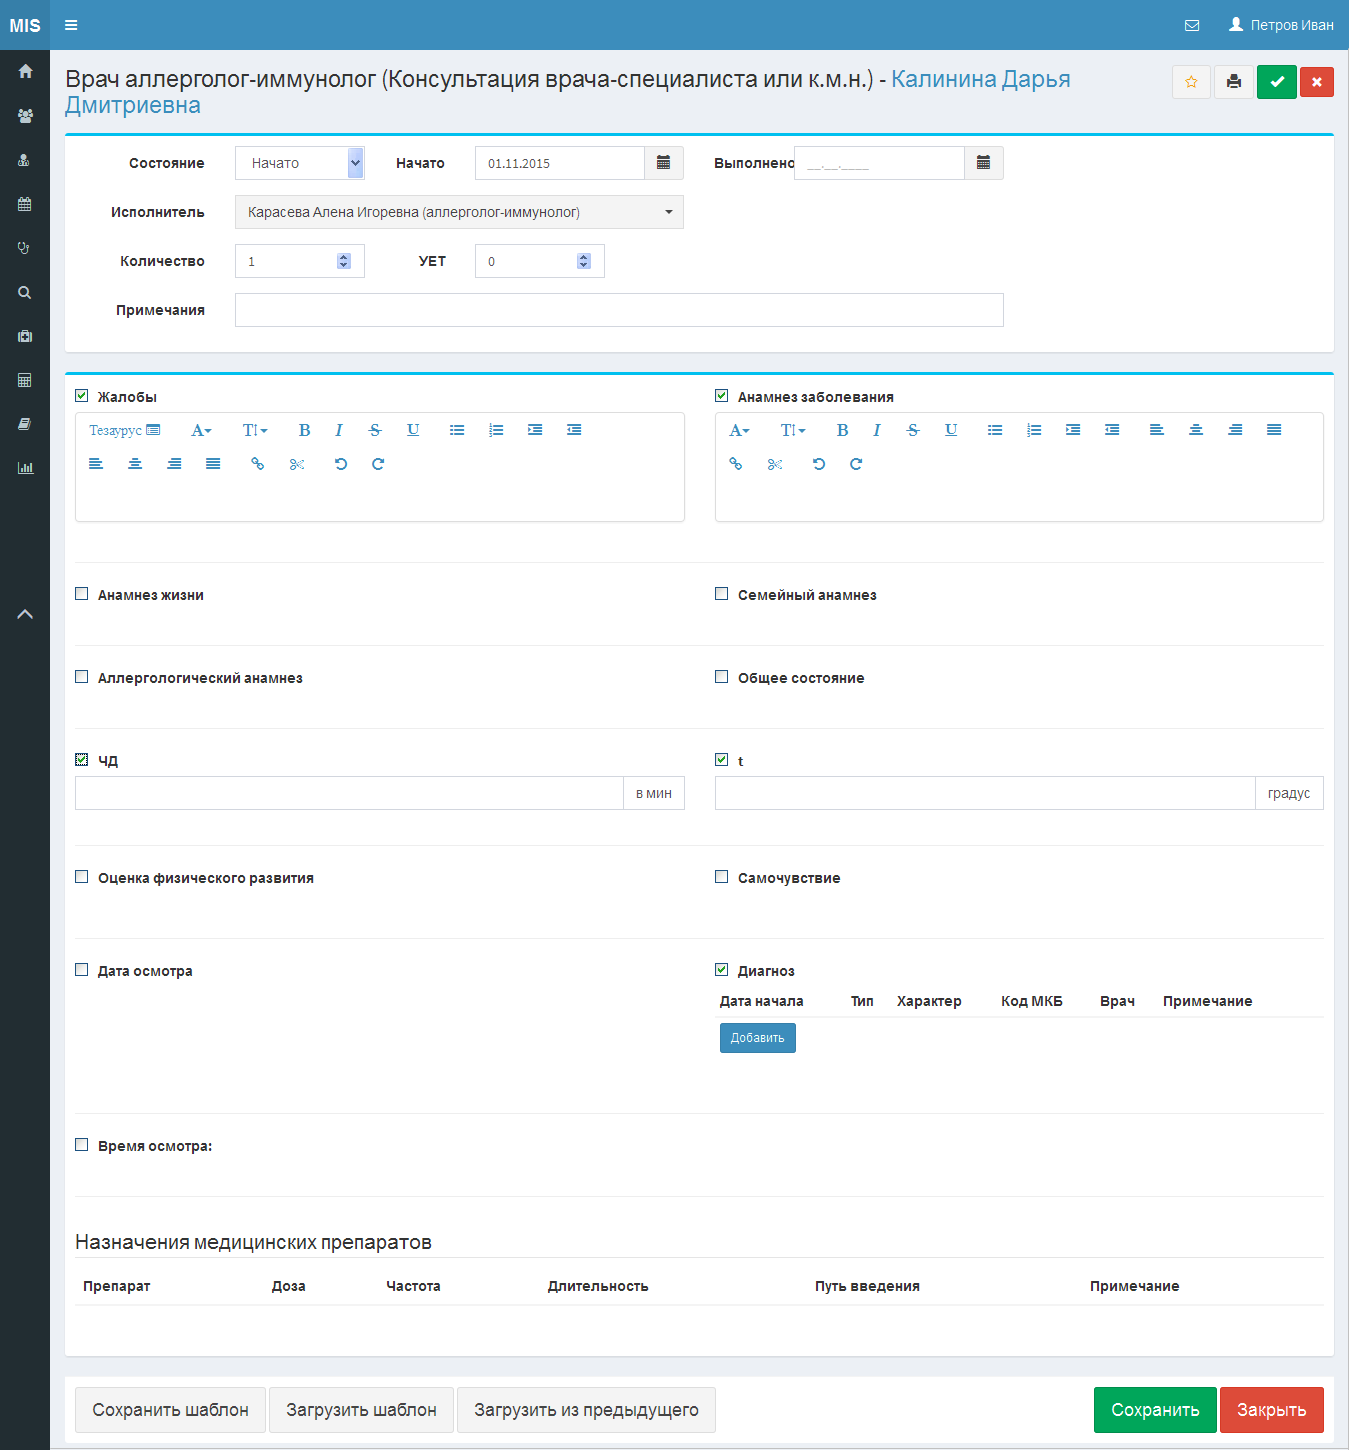
\includegraphics[width = 1\textwidth ,keepaspectratio]{ev_obr_mdedt}
 \caption{Редактирование медицинского документа}
 \label{img_ev_obr_mdedt}
\end{figure}

Название указывается в верху страницы редактирования медицинской записи и содержит название документа и фамилию пациента, для которого он создан. Эти поля недоступны для редактирования. Далее размещается ряд полей, содержащих учетные данные документа: 
\begin{itemize}
 \item \dm{Состояние} -- выбирается из справочника. Для медицинских документов доступно 2 состояния: <<Начато>> и <<Закончено>>. Как правило, документы создаются в состоянии <<Начато>>. После того, как оформление документа полностью завершено, необходимо изменить его статус на <<Закончено>> и сохранить изменения. При установке значения <<Закончено>> в данном поле, в поле \dm{Выполнено} автоматически устанавливается текущая дата. 
 \item \dm{Начато} -- дата начала документа. При создании документа в данном поле автоматически указывается текущая дата.
 \item \dm{Выполнено} -- дата завершения работы с документом. При установлении значения в данном поле, состояние документа автоматически изменяется на <<Закончено>>. 
 \item \dm{Исполнитель} -- врач, выполнивший осмотр \slash консультацию \slash дигностическое или лабораторное исследование. По умолчанию при созданнии документа в качестве исполнителя указывается текущий пользователь, но он может быть изменен путем выбора из справочника сотрудников. 
 \item \dm{Количество} -- количество назначенных процедур \slash услуг. Для большинства медицинских записей в данном поле всегда должно быть значение <<1>> (устанавливается автоматически). Исключения составляют физиотерапевтические и другие лечебно-профилактические процедуры, которые назначаются сериями по несколько процедур. 
 \item \dm{УЕТ} -- количество УЕТ для данной услуги. Как правило, значение заполняется только для стоматологических услуг.
 \item \dm{Примечание} -- дополнительные комментарии.
\end{itemize}

Описанные выше поля присутствуют во всех медицинских записях в системе. Состав полей верхней части страницы может незначительно отличаться и определяется настройками системы.

Для инструментально-диагностических и лабораторных исследований учетные данные содержат следующие дополнительные поля: 
\begin{itemize}
 \item \dm{Назначено} -- дата назначения исследования. При создании направления в данном поле по умолчанию устанавливается текущая дата;
 \item \dm{План} -- планируемая дата выполнения. При создании направления по умолчанию в данном поле указывается следующий рабочий день;
 \item Флажок \dm{Срочно} указывает, что исследование необходимо выполнить по CITO;
 \item \dm{Назначил} -- врач, назначивший исследоание, выбирается из справочника. При создании направления в данном поле по умолчанию указывается текущий пользователь.  
\end{itemize}

Остальную часть страницы занимает основная часть документа, содержащая медицинскую информацию. Поля размещаются в 2 столбца. Состав полей, их последовательность и способы заполнения различны для каждого типа документа, полностью определяются настройками системы и могут определяться каждым ЛПУ по своему усмотрению.  

Флажки слева от наименования полей определяют видимость поля на экране. Если флажок установлен, то поле отображается на экране. Для того чтобы скрыть поле, необходимо снять флажок. Если поле является обязательным для заполнения, скрыть его невозможно. Все остальные поля основной части документа доступны для скрытия и отображения. 

\begin{prim}
Установленные пользователем настройки видимости полей распространяются только на текущий экземпляр документа. Следующий документ будет создан с настройками видимости полей по умолчанию.
\end{prim}

\begin{vnim}
Скрытие поля в документе НЕ приводит к очистке информации из него. Если в поле было заполнено, а затем скрыто, то при направлении документа на печать, информация из скрытого поля попадет в печатную форму. 
\end{vnim}

В системе существуют следующие типы полей:
\begin{enumerate}
 \item \textbf{Ввод произвольного форматированного текста} (поля \dm{Жалобы} и \dm{Анамнез заболевания} на рисунке \ref{img_ev_obr_mdedt}). Предоставляет наиболее широкие возможности по вводу и редактированию текста: можно ввести в поле текст произвольной длины, задать для него шрифт, выравнивание и прочее форматирование. 
 
 В некоторых полях доступен тезаурус, содержащий основной набор фраз, использующихся при заполнении данного поля. Для вызова тезауруса необходимо нажать кнопку 
\includegraphics[scale=0.9]{edt_teza} в левом верхнем углу соответствующего поля. В результате, в правой части страницы раскроется тезаурус (Рисунок \ref{img_ev_obr_edtmd1}). В верхней части раскрывшегося всплывающего окна расположено поле редактирования. Оно дублирует основное поле ввода. Информация, введенная в это поле, после закрытия тезауруса будет скопирована в поле, из которого он был вызван. Редактирование и форматирование текста можно осуществлять как в данном окне, так и в исходном поле. Основную часть панели тезауруса занимает список фраз. Для добавления фразы в поле ввода достаточно щелкнуть по ней левой кнопкой мыши. Если список фраз тезауруса достаточно большой и не умещается на экране, для перемещения по нему следует пользоваться полосой прокрутки на правой границе окна либо колесом прокрутки мыши. После завершения работы с тезаурусом данного поля, нужно закрыть его, нажав кнопку 
\includegraphics[scale=0.9]{edt_teza_cl} в правом верхнем углу либо щелкнув левой кнопкой мыши по затененной области вне окна тезауруса. 
 
  \begin{figure}[ht!]\centering
   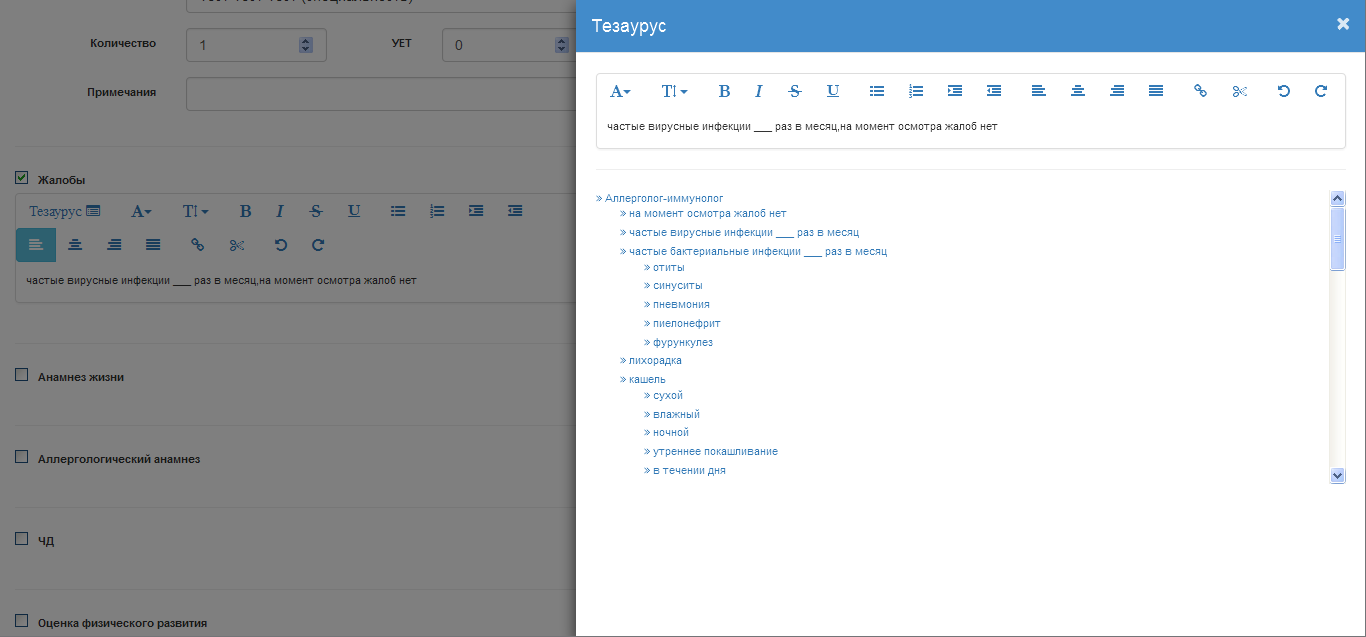
\includegraphics[width = 1\textwidth ,keepaspectratio]{ev_obr_edtmd1}
   \caption{Заполнение документа с помощью тезауруса}
   \label{img_ev_obr_edtmd1}
  \end{figure}
  
 Кроме того, в полях данного типа доступны следующие кнопки форматирования:
 
 \begin{itemize}
  \item 
\includegraphics[scale=0.9]{edt_font} -- выбор шрифта текста. При нажатии на указанную кнопку раскрывается список доступных шрифтов, из которого можно выбрать наиболее подходящий;
  \item 
\includegraphics[scale=0.9]{edt_size} -- выбор размера шрифта. При нажатии на указанную кнопку раскрывается список доступных размеров, из которого можно выбрать наиболее подходящий; 
  \item 
\includegraphics[scale=0.9]{edt_b} -- жирный шрифт; 
  \item 
\includegraphics[scale=0.9]{edt_i} -- курсив (наклонный) шрифт;
  \item 
\includegraphics[scale=0.9]{edt_s} -- зачеркнутый текст; ексто
  \item 
\includegraphics[scale=0.9]{edt_u} -- подчеркнутый текст;
  \item 
\includegraphics[scale=0.9]{edt_lm} -- создание маркированного списка;
  \item 
\includegraphics[scale=0.9]{edt_ln} -- создание нумерованного списка;
  \item 
\includegraphics[scale=0.9]{edt_pl} -- выравнивание текста по левому краю;
  \item 
\includegraphics[scale=0.9]{edt_pc} -- выравнивание текста по центру;
  \item 
\includegraphics[scale=0.9]{edt_pr} -- выравнивание текста по правому краю;
  \item 
\includegraphics[scale=0.9]{edt_pp} -- выравнивание текста по ширине страницы; 
  \item 
\includegraphics[scale=0.9]{edt_link} -- добавление гиперссылки;
  \item 
\includegraphics[scale=0.9]{edt_cut} -- удаление гиперссылки;
  \item 
\includegraphics[scale=0.9]{edt_undo} -- отмена последнего изменения;
  \item 
\includegraphics[scale=0.9]{edt_redo} -- возврат последнего отмененного изменения.      
 \end{itemize}
 
 При наличии выделенного фрагмента текста, выбранное форматирование применяется к этому фрагменту. При отсутствии выделения  форматируется текущая строка.
 
 \textbf{\item Поле со списком}, из которого можно выбрать единственное значение.
 \textbf{\item Простое поле}, в которое можно с клавиатуры ввести какое-либо значение (число, дату, строку). Тип вводимой информации определяется настройками системы. Невозможно ввести в такое поле, например, дату, если согласно настройкам ожидается ввод числового значения (Поле \dm{Температура} на рисунке \ref{img_ev_obr_mdedt}). 
 \textbf{\item Поле для ввода диагнозов пациента} представляет собой целый подраздел по работе с диагнозами пациента. Здесь может быть добавлен один или несколько диагнозов, относящихся к текущей медицинской записи. Для добавления диагноза необходимо нажать кнопку \btn{Добавить}. Кнопка расположена под списком диагнозов пациента и видна, если установлен флажок отображения для данного поля и документ доступен для редактирования текущему пользователю. После нажатия кнопки появляется новое всплывающее окно (Рисунок \ref{img_ev_obr_mdedtdiag}) , где следует указать следующие сведения о диагнозе: 
 \begin{itemize}
  \item \dm{Тип} -- тип диагноза выбирается из справочника. Поле является обязательным для заполнения;
  \item \dm{Дата начала} -- дата установления диагноза. Поле является обязательным для заполнения;
  \item \dm{Дата окончания} -- дата снятия диагноза;
  \item \dm{МКБ} -- код диагноза согласно справочник МКБ-10. Код выбирается из справочника (см. раздел \ref{gen_filtr}). В справочнике предусмотрен поиск как по коду (или его части), так и по названию заболевания. Поле является обязательным для заполнения.
  \item \dm{Характер} -- характер заболевания выбирается из справочника;
  \item \dm{Врач} -- врач, установивший диагноз. Значение выбирается из справочника. По умолчанию в качестве врача указывается текущий пользователь. Поле является обязательным для заполнения.
  \item \dm{Результат} -- результат лечения заболевания;
  \item \dm{Исход} -- исход заболевания;
  \item \dm{Описание диагноза} -- в данное поле можно ввести расширенное (по сравнению со справочником МКБ-10) описание диагноза. 	  	 	    
 \end{itemize} 
 
  \begin{figure}[ht!]\centering
    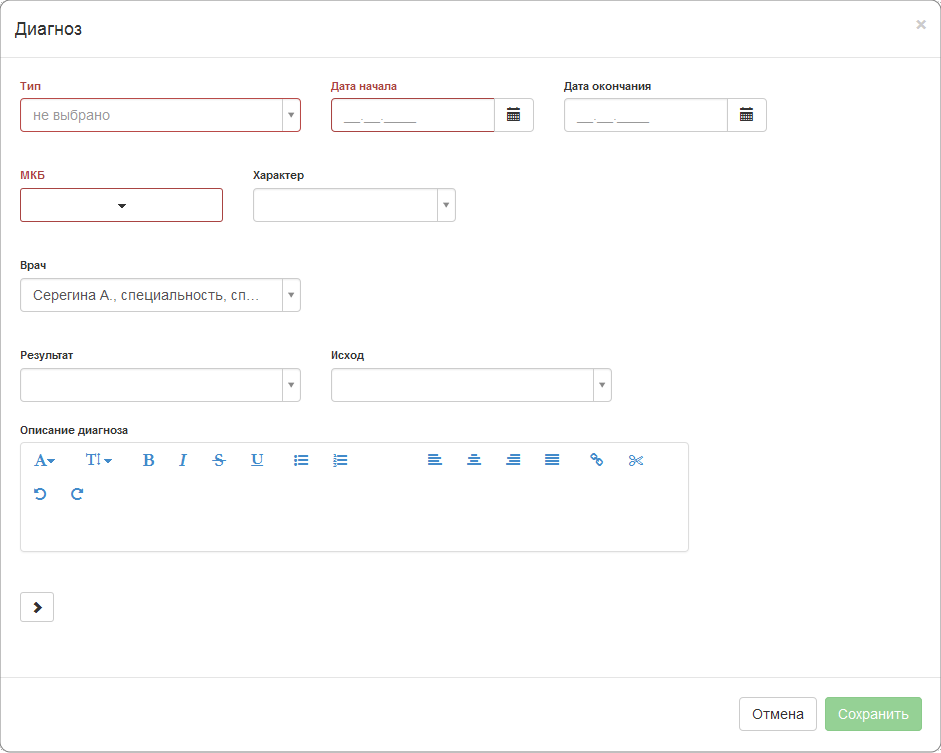
\includegraphics[width = 1\textwidth ,keepaspectratio]{ev_obr_mdedtdiag}
    \caption{Регистрация диагноза пациента}
    \label{img_ev_obr_mdedtdiag}
  \end{figure}
  
 При нажатии на кнопку 
\includegraphics[scale=0.6]{rolldown}, расположенную в нижней части всплывающего окна, раскроется ряд полей для ввода дополнительных сведений о диагнозе (Рисунок \ref{img_ev_obr_mdedtdiag2}):
 \begin{itemize}
  \item \dm{Фаза} -- фаза онкологического заболевания, выбирается из справочника;
  \item \dm{Стадия} -- стадия заболевания, выбирается из справочника;
  \item \dm{Травма} -- вид травмы, ставшей причиной заболевания, выбирается из справочника;
  \item \dm{Группа здоровья} -- группа здоровья пациента, выбирается из справочника;
  \item \dm{Диспансерное наблюдение} -- признак постанови или снятия с диспансерного учета по данному заболеванию, выбирается из справочника;
  \item \dm{Примечание} -- дополнительные комментарии.
 \end{itemize}
 
   \begin{figure}[ht!]\centering
   	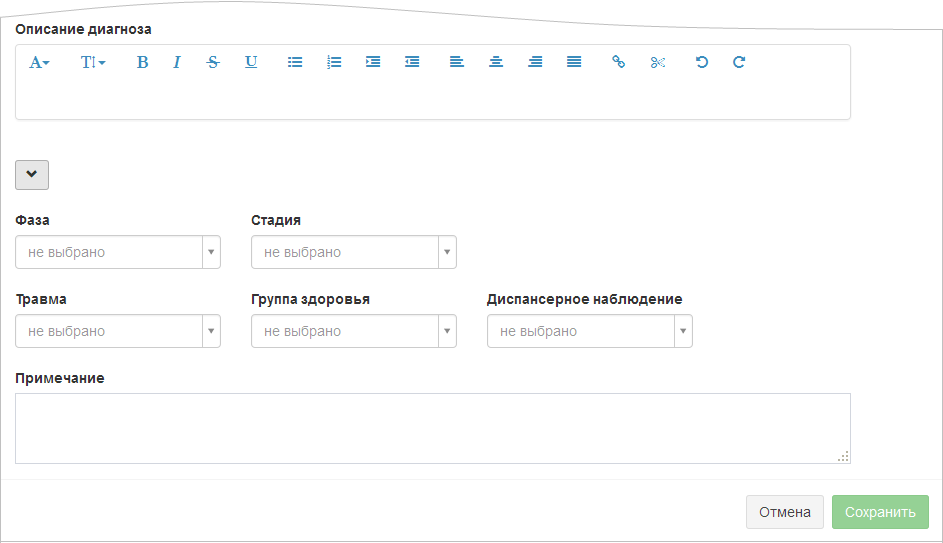
\includegraphics[width = 1\textwidth ,keepaspectratio]{ev_obr_mdedtdiag2}
   	\caption{Расширенные характеристики диагноза}
   	\label{img_ev_obr_mdedtdiag2}
   \end{figure}
   
 После того как все необходимые поля сведений о диагнозе заполнены, нужно нажать кнопку \btn{Сохранить} в правом нижнем углу всплывающего окна \dm{Диагноз}. Если какие-либо из обязательных полей не заполнены, кнопка будет неактивна. Если кнопка не видна на экране, следует переместиться в конец страницы, воспользовавшись колесом прокрутки мыши или полосой прокрутки на экране. После успешного сохранения диагноз будет добавлен на страницу медицинского документа (Рисунок \ref{img_ev_mdedtd}) и в раздел \dm{Диагнозы} карточки обращения. Запись о диагнозе может быть удалена или отредактирована, пока медицинский документ находится в состоянии <<Начато>>. Для удаления записи необходимо нажать кнопку 
\includegraphics[scale=0.6]{del} справа от записи, для редактирования -- кнопку 
\includegraphics[scale=0.6]{edt}. 
  
\end{enumerate}
 
  \begin{figure}[ht!]\centering
  	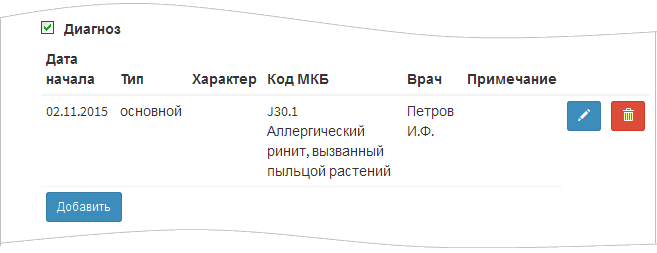
\includegraphics[width = 1\textwidth ,keepaspectratio]{ev_obr_mdedtd}
  	\caption{Регистрация диагнозов пациента в медицинском документе}
  	\label{img_ev_mdedtd}
  \end{figure}
  
Заполнив описанными выше методами все поля медицинского документа, следует сохранить его. Для этого нужно нажать кнопку \btn{Сохранить} в правом нижнем углу страницы либо кнопку 
\includegraphics[scale=0.6]{ok} в правом верхнем углу. После возврата на страницу обращения в разделе \dm{Медицинские документы} появится новая запись. Кнопка \btn{Закрыть} или 
\includegraphics[scale=0.6]{xdel} закрывает страницу редактирования документа без сохранения.

\paragraph{Печать документов}

Для вывода на печать полученного документа нужно нажать кнопку 
\includegraphics[scale=0.6]{print} в правом верхнем углу страницы, в появившемся всплывающем окне (Рисунок \ref{img_ev_mdpirnt}) установить флажки напротив тех форм, которые необходимо вывести на печать и нажать кнопку \btn{Печать}. Откроется окно предварительного просмотра печати выбранных документов с возможностью отправки на принтер. Кнопка \btn{Печать компактно} выводит документы на печать без разделителей страниц.

 \begin{figure}[ht]\centering
   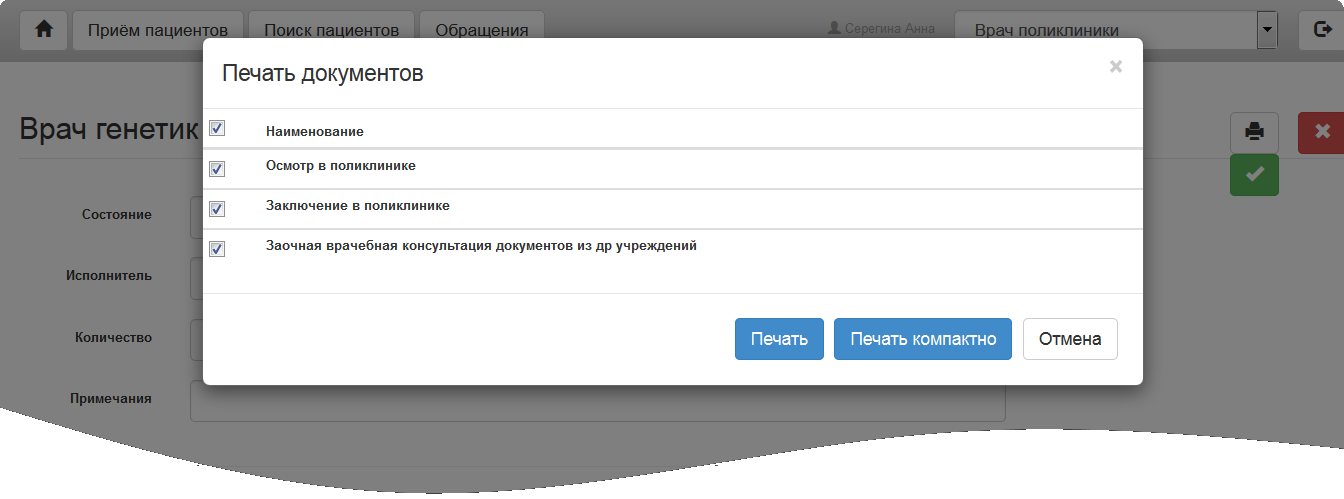
\includegraphics[width = 0.7\textwidth ,keepaspectratio]{ev_mdprint}
   \caption{Выбор печатных форм медицинского документа}
   \label{img_ev_mdpirnt}
 \end{figure}
  
\paragraph{Просмотр и редактирование медицинских записей. Состояния}

В зависимости от состояния, медицинская запись может открываться для редактирования либо просмотра. Внешний вид документа, открытого на редактирование, представлен на рисунке \ref{img_ev_obr_mdedt}. Внешний вид документа, открытого для просмотра, представлен на рисунке \ref{img_ev_mdview}.

 \begin{figure}[ht]\centering
   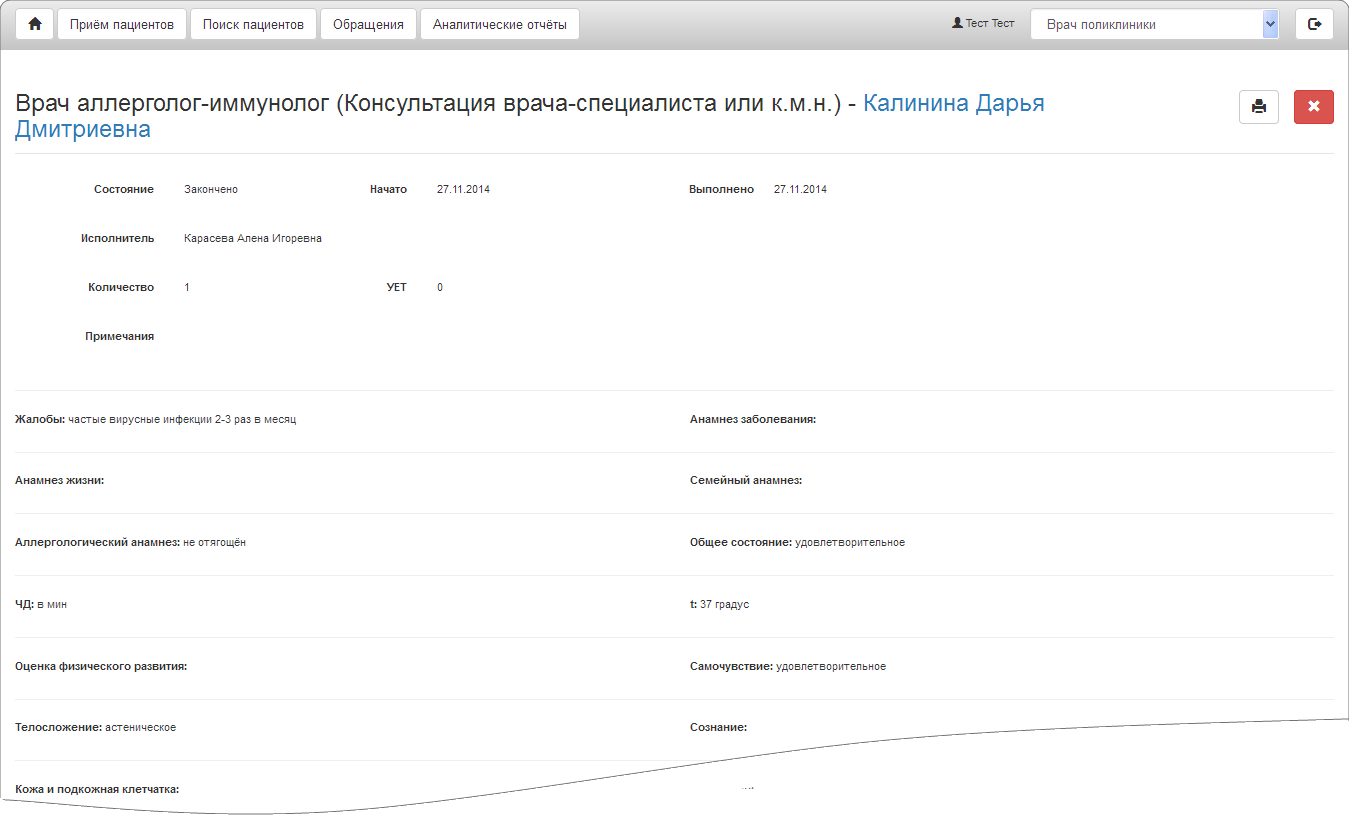
\includegraphics[width = 1\textwidth ,keepaspectratio]{ev_mdview}
   \caption{Просмотр медицинского документа}
   \label{img_ev_mdview}
 \end{figure}

Доступность для редактирования определяется:
\begin{enumerate}
 \item Наличием у пользователя прав на редактирование медицинских записей данного типа;
 \item Состоянием медицинской записи (см. подробное описание ниже);
 \item Состоянием обращения, в состав которого входит медицинская запись. Если обращение закрыто, то все медицинские записи, входящие в него, недоступны для редактирования.  
\end{enumerate} 

Медицинские записи могут находиться в двух состояниях:
\begin{itemize}
 \item Начато -- документ находится в работе. Данное состояние устанавливается при создании документа. Документы в данном состоянии доступны для редактированиия (при наличии у пользователя соответствующих прав) и удаления. 
 \item Закончено -- оформнение документа завершено. Запись о таком документе на странице обращения выделена зеленым цветом. Удаление и редактирование документов в состоянии <<Закончено>> невозможно. Устанавливать документу состояние <<Закончено>>   следует только после того, как работа над ним полностью завершена. При указании даты выполнения в документе, ему автоматически присваивается состояние  <<Закончено>>. 
\end{itemize}


\ifthenelse{\NOT \isnamedefined{diagnversion}}
{
\subsubsection{Медицинские документы} \label{ev_obr_md}

В данном разделе можно просмотреть, добавить или отредактировать результаты консультаций\slash осмотров врачей по выбранному случаю обращения (Рисунок \ref{img_ev_obrmd}) и другие медицинские документы пациента.

\begin{figure}[ht]\centering
 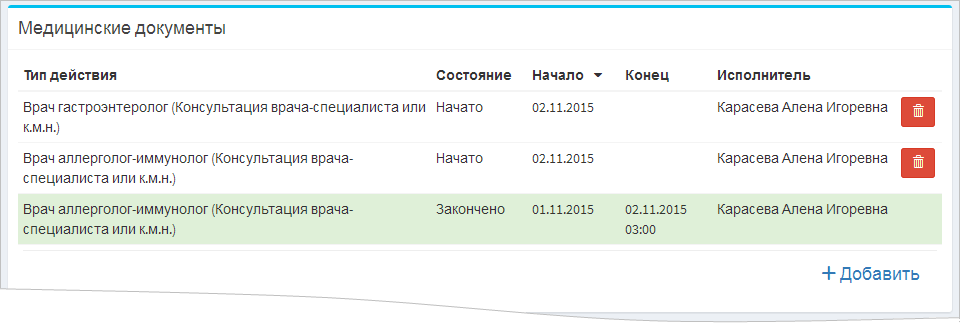
\includegraphics[width = 1\textwidth ,keepaspectratio]{ev_obrmd}
 \caption{Карточка редактирование обращения. Раздел <<Медицинские документы>>}
 \label{img_ev_obrmd}
\end{figure}
}{}

Механизмы работы с медицинскими документами полностью соответствует описанной в разделе \ref{pol_obr_gen}

\subsubsection{Раздел «Диагностика»} \label{ev_obr_is}

\ifthenelse{\NOT \isnamedefined{diagnversion}}
{
В данном разделе (Рисунок \ref{img_ev_obr_isedt}) существует возможность:
\begin{itemize}
 \item регистрации направлений на инструментальные диагностические исследования;
 \item просмотра зарегистрированных направлений и результатов выполненных исследований;
 \item ввода результатов исследований.
\end{itemize}
 
\paragraph{Создание направлений на диагностические исследования}

Для добавления нового направления на инструментально-диагностическое исследование необходимо нажать кнопку  \btn{Создать} в конце раздела. Далее следует выбрать тип исследования и создать направление аналогично созданию медицинского документа (см. раздел \ref{ev_obr_md})

Внешний вид (Рисунок \ref{img_ev_obr_isedt}) и принцип заполнения страницы инструментально-диагностических исследований аналогичен описанному в разделе (\ref{ev_obr_mdedt}).

При создании направления необходимо заполнить следующие поля:

\begin{itemize}
 \item \dm{Назначено};
 \item \dm{План};
 \item Установить флажок \dm{Срочно} при необходимости;
 \item \dm{Назначил}.
\end{itemize}

}{}

 \begin{figure}[ht]\centering
   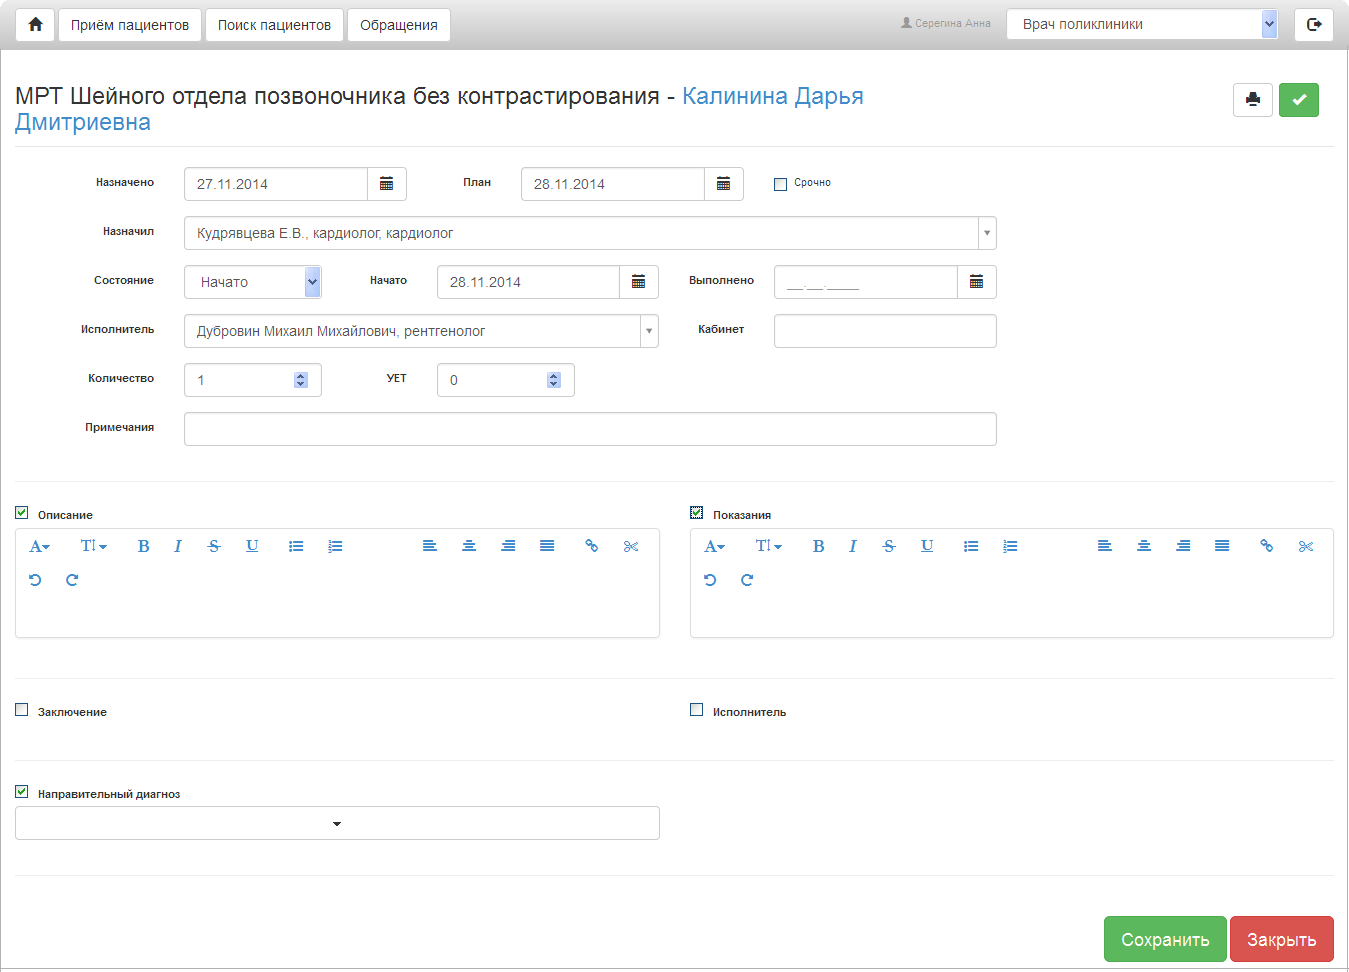
\includegraphics[width = 1\textwidth ,keepaspectratio]{ev_obr_isedt}
   \caption{Страница диагностичиеского исследования}
   \label{img_ev_obr_isedt}
 \end{figure}  

\ifthenelse{\NOT \isnamedefined{diagnversion}}
{ 
Так же может потребоваться заполнение некоторых полей основной части документа в части направительных данных, такие как диагноз направления, показания для проведения исследования и т.п. Остальные поля заполняются врачом, выполняющим диагностическое исследование.

После того как все необходимые поля заполнены, нужно сохранить направление. Для этого нужно нажать кнопку \btn{Сохранить} в правом нижнем углу страницы либо кнопку 
\includegraphics[scale=0.6]{ok} в правом верхнем углу. После возврата на страницу обращения в разделе \dm{Диагностика} появится соответствующая запись. Кнопка \btn{Закрыть} закрывает страницу редактирования направления без сохранения.
}
{
В данном разделе должны регистрироваться результаты диагностических исследований пациента. Как правило, направления на диагностические исследования создаются врачами-специалистами или в регистратуре. Но при необходимости, врач диагностики сам может зарегистрировать новое исследование. Для этого нужно нажать кнопку \btn{Создать} в разделе \dm{Диагностика} карточки обращения, выбрать вид исследования (см. раздел \ref{img_ev_obr_addmd}) и заполнить учетные данные в верхней части открывшейся страницы (см. раздел \ref{img_ev_obr_isedt}) 

Сразу же после этого можно приступить к заполнению результатов исследования (см. раздел \ref{ev_obr_isrez})
}

\ifthenelse{\NOT \isnamedefined{doctorversion}}
{
\paragraph{Ввод результатов функциональной диагностики} \label{ev_obr_isrez}

Для ввода результатов инструментально-диагностического исследования необходимо открыть страницу исследования на редактирование, щелкнув левой кнопкой мыши по соответствующей записи в разделе \dm{Диагностика} карточки обращения. Если у пользователя достаточно прав для редактирования документа и документ находится в состоянии <<Начато>>, страница диагностического исследования откроется для редактирования (Рисунок \ref{img_ev_obr_isedt}). 

Ввод результатов исследований состоит из 2-х этапов: заполнение учетных данных и заполнение медицинской информации в основной части документа.

При вводе результатов исследования необходимо заполнить следующие поля раздела учетных данных:
\begin{itemize}
 \item \dm{Состояние} –- выбирается из списка. После того, как  исследование выполнено, необходимо перевести его в состояние <<Закончено>>. При установке в данном поле состояния <<Закончено>>, в поле \dm{Ваполнено} автоматически устанавливается текущая дата.
 \item \dm{Начато} –- дата начала выполнения, заполняется автоматически в момент создания направления и устанавливается равной текущей дате. Если исследование выполняется в другой день, то следует изменить дату начала;
 \item \dm{Выполнено} -– дата завершения выполнения. При изменении значения в поле \dm{Состояние} на <<Закончено>>, в данном поле автоматически устанавливается текущая дата;
 \item \dm{Исполнитель} -– фамилия специалиста, выполнившего исследование, выбирается из справочника;
 \item \dm{Кабинет} –- номер кабинета, в котором было выполнено исследование;
 \item \dm{УЕТ} –- как правило, заполняется только для стоматологических услуг;
 \item \dm{Количество} -- количество выполненных исследований данного вида. Как правило, в поле устанавливается значение <<1>>.
 \item \dm{Примечание} –- дополнительная информация.
\end{itemize}

Принцип заполнения основной части документа аналогичен описанному в разделе \ref{ev_obr_mdedt}

% При наличии на диагностическом оборудовании возможности создавать архив результатов исследований в формате DICOM, можно организовать связь с результатами пациента. Тогда врач сможет воспользоваться этой связью и просмотреть результат пациента. Для создания связи необходимо нажать кнопку \btn{DICOM Архив} в правой нижней части окна и из открывшегося меню выбрать пункт \dm{Сопоставить с DICOM Архивом}. Откроется диалоговое окно, где необходимо указать имя или номер файла и нажать кнопку \btn{Сохранить}.

% Для просмотра связанного DICOM-файла результата, нужно нажать кнопку \btn{DICOM Архив} в правой нижней части окна и из открывшегося меню выбрать пункт \btn{Просмотр на DICOM Архиве}. После этого откроется окно просмотра результата исследования в формате DICOM.

% Если связь с DICOM-файлом была создана ошибочно, можно разорвать ее, нажав кнопку \btn{DICOM Архив} в правой нижней части окна и выбрав пункт \dm{Отменить сопоставление с DICOM Архивом}. После разрыва связи, можно создать связь с правильным файлом.

Для вывода на печать полученного документа нужно нажать кнопку \includegraphics[scale=0.6]{print} в правом верхнем углу страницы, в появившемся всплывающем окне (Рисунок \ref{img_ev_isprint}) установить флажки напротив тех форм, которые необходимо вывести на печать и нажать кнопку \btn{Печать}. Откроется окно предварительного просмотра печати выбранных документов с возможностью отправки на принтер. Кнопка \btn{Печать компактно} выводит документы на печать без разделителей страниц.

 \begin{figure}[ht]\centering
   \includegraphics[width = 0.7\textwidth ,keepaspectratio]{ev_isprint}
   \caption{Выбор печатных форм диагностического исследования}
   \label{img_ev_isprint}
 \end{figure}
}{}
 
\paragraph{Редактирование направлений на диагностические исследования} \label{ev_obr_isedt}

Для редактирования направления на инструментально-диагностическое исследование нужно щелкнуть левой кнопкой мыши по соответствующей записи в разделе \dm{Диагностика}. Если у пользователя достаточно прав для редактирования документа и документ находится в состоянии <<Начато>>, страница диагностического исследования откроется для редактирования (Рисунок \ref{img_ev_obr_isedt}) и можно будет добавить или изменить данные направления.

Для сохранения изменений данных необходимо нажать кнопку \btn{Сохранить}.

Для удаления направления нужно нажать кнопку \includegraphics[scale=0.6]{del} напротив соответствующей записи в разделе \dm{Диагностика} на странице обращения. Удаление неправления возможно только, если исследование еще не выполнено, т.е. документ находится в состоянии <<Начато>>.

\subsubsection{Раздел <<Лаб.исследования>>}

В данном разделе можно просмотреть, добавить или отредактировать направления на лабораторные исследования и их результаты (Рисунок \ref{img_ev_obrlab}).

\begin{figure}[ht]\centering
 \includegraphics[width = 1\textwidth ,keepaspectratio]{ev_obrlab}
 \caption{Карточка обращения. Раздел <<Лаб.исследования>>}
 \label{img_ev_obrlab}
\end{figure}

Документы  в разделе \dm{Лаб.исследования} могут находиться в следующих состояниях:
\begin{itemize}
 \item Начато -- документ создан, но не закрыт. Документы в данном состоянии доступны для редактированиия (при наличии у пользователя соответствующих прав) и удаления. 
 \item Ожидание -- исследуемый материал направлен на исследование. Ожидание ответа от автоматического анализатора. Данное состояние может возникать только при организации взаимодействия \tmis с лабораторной системой ЛПУ.
 \item Закончено -- оформнение документа завершено. Результаты исследования внесены в документ вручную или получен ответ от анализатора. Запись о таком документе на странице обращения выделена зеленым цветом. Удаление документов в статусе <<Закончено>> невозможно.
 \item Отменено -- выполнение исследования отменено.
 \item Без результата -- не удалось получить результат от автоматического анализатора \slash ошибка при получении результата.
\end{itemize}

\paragraph{Создание направления на лабораторное исследование}

Если обращение не закрыто и при наличии у пользователя соответствующих прав, можно зарегистрировать новое направление на лаборатрное исследование. Для этого нужно нажать на кнопку \btn{Создать} в конце раздела \dm{Лаб.исследования}, появится новое всплывающее окно, содержащее дерево типов лабораторных исследований (Рисунок \ref{img_ev_obr_addlab}).

\begin{figure}[ht]\centering
 \includegraphics[width = 1\textwidth ,keepaspectratio]{ev_obr_addlab}
 \caption{Создание направления на лабораторное исследование}
 \label{img_ev_obr_addlab}
\end{figure}

В дереве присутствуют группы и виды исследований. Виды исследований слева помечены значком с изображением желтой папки. Их можно выбрать для создания направления. Группы исследований предназначены только для систематизации видов исследований и удобства поиска. Они имеют слева знак <<$+$>> (если группа свернута) или <<$-$>> (если группа раскрыта). При нажатии на наименование группы она меняет свое состояние (сворачивается или разворачивается в зависимости от предыдущего состояния). По умолчанию дерево видов исследований полностью развернуто. 

В верхней части окна находится поле поиска. При вводе текста в него, осуществляется фильтрация видов исследований в дереве -- отображаются только виды, в наименовании которых встречается введенное буквосочетание и группы, содержащие их. Остальные  группы и виды исследований скрываются. Фильтрация производится аналогично другим справочникам системы (см. раздел \ref{gen_filtr}). 

%Флажок \dm{Только разрешенные в моем отделении} ограничивает список категорий лишь теми, которые разрешены в отделении к которому прикреплен пользователь. При необходимости можно снять данный флажок тогда список будет содержать все категории документов, доступные для создания данным пользователем.

%Флажок \dm{Только разрешенные мне} ограничивает список категорий лишь теми, которые разрешены текущему пользователю. При необходимости можно снять данный флажок тогда список будет содержать все категории документов, доступные для создания данным пользователем.

\begin{prim}
 Для облегчения поиска список доступных категорий исследований для конкретного пользователя (или группы пользователей) может быть ограничен настройками системы. Если в списке отсутствует тип лабораторных исследований, необходимый для работы, следует обратиться к администратору системы.
\end{prim} 

Для создания направления необходимо щелкнуть левой кнопкой мыши по наименованию соответствующего вида исследований. В результате, выбранное наименование появится в правой части окна. Допускается выбор сразу нескольких видов лабораторных исследований для последующего пакетного создания направлений. Для выбранных исследований можно задать:

\begin{enumerate}
 \item Набор параметров для исследования. Для этого необходимо щелкнуть левой кнопкой мыши по наименованию выбранного исследования в правой части окна и в новом всплывающем окне (Рисунок \ref{img_ev_obr_labpar}) оставить флажки только для тех параметров, которые необходимо исследовать. При снятии флажка \dm{Выбрать все} в верхней части окна, снимаются флажки со всех параметров. При установке данного флажка, устанавливаются флажки для всех параметров выбранного исследования.
 \item Планируемые дату и время выполнения исследования. Для этого следует выбрать нужную дату и время в полях \dm{Дата \slash время назначения}. В созданном направлении в поле \dm{План} будет указана выбранная дата. 
 \item Удалить исследование из списка выбранных к назначению, нажав кнопку \includegraphics[scale=0.6]{del} справа от наименования соответствующего типа исследований.
\end{enumerate}

 \begin{figure}[ht]\centering
 	\includegraphics[width = 0.7\textwidth ,keepaspectratio]{ev_obr_labpar}
 	\caption{Выбор параметров исследования}
 	\label{img_ev_obr_labpar}
 \end{figure}
 
После того как список необходимых направлений на лабораторные исследования сформирован и все параметры заданы, нужно нажать кнопку \btn{Создать направления} в правом нижнем углу всплывающего окна. Выбранные типы исследований будут добавлены в раздел \dm{Лаб.исследования} карточки обращения.

\paragraph{Редактирование направления на лабораторное исследование}

Для редактирования данных направления на лабораторное исследование необходимо открыть страницу исследования для редактирования, щелкнув левой кнопкой мыши по его наименованию в разделе \dm{Лаб. исследования} карточки обращения. Откроется страница лабораторного исследования (Рисунок \ref{img_ev_obrlab}). Редактирование данных направления на исследование возможно только в состоянии <<Начато>>.

В верхней части страницы указываются учетные данные лабораторного исследования. Часть из них заполняется при создании направления, остальные -- при выполнении исследования. Можно внести данные либо изменить значения в следующих полях:

\begin{itemize}
 \item \dm{Назначено} -- дата назначения исследования. При создании направления в данном поле по умолчанию устанавливается текущая дата или дата исследования, указанная при создании направления;
 \item \dm{План} -- планируемая дата выполнения исследования. При создании направления по умолчанию в данном поле указывается следующий рабочий день за датой назначения;
 \item Флажок \dm{Срочно} указывает, что исследование необходимо выполнить по CITO;
 \item \dm{Назначил} -- врач, назначивший исследование, выбирается из справочника. При создании направления в данном поле по умолчанию указывается текущий пользователь.  
\end{itemize} 

В основной части документа нужно указать направительный диагноз в случае наличия такого поля для выбранного типа исследования, выбрав его из справочника МКБ-10. Так же можно изменить набор назначаемых параметров исследования. Для этого нужно снять или установить флажки напротив параметров в столбце \dm{Назначено}. Флажки должны быть установлены только для тех параметров, которые необходимо исследовать.  

После внесения всех необходимых изменений, требуется сохранить корректировки, нажав кнопку \btn{Сохранить} в правом нижнем углу страницы либо кнопку \includegraphics[scale=0.6]{ok} в правом верхнем углу.    

Для удаления направления нужно нажать кнопку \includegraphics[scale=0.6]{del} напротив соответствующей записи в разделе \dm{Лаб.исследования} на странице обращения. Удаление неправления возможно только, если исследование еще не выполнено, т.е. документ находится в состоянии <<Начато>>.

\ifthenelse{\isnamedefined{fullversion}}
{
\paragraph{Ввод результатов лабораторных исследований} \label{ev_obr_rez}
 
В данном разделе будет рассмотрена методика работы врача по вводу единичных результатов лабораторных исследований. Потоковый ввод результатов лабораторных исследований выполняется в специальном разделе.

Для ввода результатов лабораторного исследования необходимо открыть направление на редактирование, щелкнув левой кнопкой мыши по его наименованию в разделе \dm{Лаб. исследования} карточки обращения. Откроется страница лабораторного исследования (Рисунок \ref{img_ev_obrlab}). 

В верхней части страницы нужно заполнить следующие поля: 

\begin{itemize}
 \item \dm{Состояние} – выбирается из списка. После того, как  исследование выполнено, необходимо перевести его в состояние <<Закончено>>. При установке в данном поле состояния <<Закончено>>, в поле \dm{Выполнено} автоматически устанавливается текущая дата.
 \item \dm{Начато} – дата начала выполнения, заполняется автоматически в момент создания направления и устанавливается равной текущей дате;
 \item \dm{Выполнено} – дата завершения выполнения. При изменении значения в поле \dm{Состояние} на <<Закончено>>, в данном поле автоматически устанавливается текущая дата;
 \item \dm{Исполнитель} – фамилия специалиста, выполнившего исследование, выбирается из справочника;
 \item \dm{Кабинет} – номер кабинета, в котором было выполнено исследование;
 \item \dm{УЕТ} – как правило, заполняется только для стоматологических услуг;
 \item \dm{Примечание} – дополнительная информация.
\end{itemize}

В основной части документа данные представлены в виде таблицы, содержащей следующие столбцы: 

\begin{itemize}
 \item В первом столбце указывается наименование параметра исследования;
 \item В столбце \dm{Назначено} флажками отмечены параметры исследования, которые необходимо выполнить;
 \item \dm{Значение} -- единственный столбец, который заполняется при вводе результатов исследования. Значения следует указывать только для параметров, у которых установлен флажок в столбце \dm{Назначено}.
 \item \dm{Ед.измерения} -- подставляется автоматически из свойств параметров исследования;
 \item \dm{Норма} -- границы нормы для значений параметра, подставляются автоматически из свойств параметров исследования.
\end{itemize}

При вводе результатов следует заполнять только поле \dm{Значение} для параметров, отмеченных флажками. После этого следует изменить значение в поле \dm{Статус анализа} основной части документа выбрать значение <<Закончен>> и сохранить данные, нажав кнопку \btn{Сохранить} в правом нижнем углу страницы либо кнопку \includegraphics[scale=0.6]{ok} в правом верхнем углу.    

После заполнения результатов исследования, его можно вывести на печать. Для этого следует нажать кнопку \includegraphics[scale=0.6]{print} в правом верхнем углу страницы, в появившемся всплывающем окне установить флажки напротив тех форм, которые необходимо вывести на печать и нажать кнопку \btn{Печать}. Откроется окно предварительного просмотра печати выбранных документов с возможностью отправки на принтер. Кнопка \btn{Печать компактно} выводит документы на печать без разделителей страниц.
}{}

\ifthenelse{\NOT \isnamedefined{diagnversion}}
{
\subsubsection{Раздел «Лечение»} \label{ev_obr_lek}

Данный раздел предназначен для регистрации направлений на медикаментозное, физиотерапевтическое, оперативное и другие виды лечения, а так же для контроля их выполнения.

Логика работы данного раздела практически полностью повторяет логику работы предыдущих разделов, поэтому приводить повторное описание работы не целесообразно.

Регистрация нового назначения аналогична описанной в разделе \ref{ev_obr_is} При регистрации нового назначения карточка лечения открывается для редактирования. Необходимо заполнить поля \dm{Дата назначения}, \dm{Срочно}, \dm{План}, \dm{Назначил}, а так же заполнить табличную часть (Рисунок \ref{img_ev_obr_lek}). Заполнение учетных данных в верхней части страницы аналогично приведенному в разделе \ref{ev_obr_isrez} Заполнение табличной части подробно описано в разделе \ref{ev_obr_mdedt}

 \begin{figure}[ht]\centering
   \includegraphics[width = 1\textwidth ,keepaspectratio]{ev_obr_lek}
   \caption{Карточка назначения лечения}
   \label{img_ev_obr_lek}
 \end{figure}
 
После того как все данные внесены, необходимо сохранить назначение, нажав кнопку \btn{Сохранить}  в правом нижнем углу страницы либо кнопку \includegraphics[scale=0.6]{ok} в правом верхнем углу.    

Для печати назначения следует нажать кнопку \includegraphics[scale=0.6]{print} в правом верхнем углу страницы, в появившемся всплывающем окне установить флажки напротив тех форм, которые необходимо вывести на печать и нажать кнопку \btn{Печать}. Откроется окно предварительного просмотра печати выбранных документов с возможностью отправки на принтер. Кнопка \btn{Печать компактно} выводит документы на печать без разделителей страниц.
}{}

\subsubsection{Закрытие случая обращения}

После того как лечение пациента по данному случаю обращения завершено, обращение необходимо закрыть. Закрытие обращения говорит о том, что активная работа с данным пациентом по данному случаю обращения завершена. После закрытия редактирование обращения и всех медицинских записей в его составе становится невозможным. Как правило, статистический учет и выставление счетов СМО производится только по закрытым обращениям.

\begin{vnim}
 Закрытие обращения выполняется без дополнительных подтверждений и является необратимой операцией! Будьте внимательны при закрытии обращений!
\end{vnim} 
 
Для успешного закрытия обращения необходимо в одном из медицинских документов указать заключительный диагноз пациента (при этом он обязательно отразится в разделе \dm{Диагнозы} на странице обращения), а так же заполнить поле \dm{Результат обращения} в разделе \dm{Основная информация}. Заполнение поля \dm{Результат обращения} является обязательным условием для закрытия обращения. Обязательность заполнения поля \dm{Исход заболевания} определяется настройками системы.

Для закрытия обращения необходимо нажать кнопку \btn{Закрыть обращение} в левой части страницы. Если данные о результате лечения не были заполнены, появится соответствующее предупреждение. Если все необходимые поля заполнены, будет произведено закрытие случая обращения и появится сообщение об успешном выполнении операции.

\subsubsection{Удаление обращения}

Если у пользователя имеются соответствующие права, обращение может быть удалено. Для этого необходимо нажать на кнопку \dm{Удалить обращение} в левой части страницы обращения и в появившемся диалоговом окне подтвердить удаление обращения, нажав кнопку \btn{Да}. Обращение будет удалено.

}{}

\subsection{Фильтрация обращений} \label{ev_obr_filtr}

Поиск и фильтрация обращений возможна в разделе \dm{Обращения}. Для перехода к разделу необходимо нажать одноименную кнопку в верхней части страницы. Откроется страница (Рисунок \ref{img_ev_filtr}), в левой части которой расположены параметры фильтрации обращений: 

\begin{itemize}
 \item \dm{Идентификатор обращения} -- поиск по номеру обращения в системе. Поиск успешен только при указании полного номера обращения в системе.
 \item \dm{Начато} -- в результаты поиска попадают обращения, дата начала которых попадает в заданный интервал. Если вторая дата в интервале не заполнена, то будет осуществлен поиск обращений, дата начала которых больше или рвна указанной в первом поле.
 \item \dm{Только незавершенные} -- результат будет включать обращения, у которых не заполнено поле \dm{Дата выполнения}.
 \item \dm{Завершено} -- результат будет включать обращения, у которых дата выполнения попадает в заданный интервал. Если дата выполнения не заполнена, обращение не будет включено в результаты фильтрации. Если вторая дата в интервале не заполнена, то будет осуществлен поиск обращений, дата завершения которых больше или рвна указанной в первом поле.
 \item \dm{Пациент} -- отображение обращений только указанного патциента. Пациент выбирается из справочника -- картотеки пациентов (см. раздел \ref{gen_filtr})
 \item \dm{Тип финансирования} -– результат будет включать только обращения с указанным типом финансирования, выбирается из справочника.
 \item \dm{Тип обращения} –- результат будет включать только обращения указанного типа, выбирается из справочника.
 \item \dm{Специальность врача} -- результат будет включать только обращения, в которых специальность врача, являющегося ответственным за обращение (лечащим врачом) соответствует указанному в поле. Значение поля выбирается из справочника.
 \item \dm{Лечащий врач} -- результат будет включать только обращения, в которых фамилия врача, ответственного за обращение (указанного в качестве лечащего в обращении) соответствует выбранной в поле.
 \item \dm{Результат} -- результат будет включать только обращения, в которых результат обращения соответствует указанному в поле. Значение поля выбирается из справочника.
\end{itemize}

\begin{figure}[ht]\centering
   \includegraphics[width = 1\textwidth ,keepaspectratio]{ev_filtr}
   \caption{Страница <<Обращения>>}
   \label{img_ev_filtr}
 \end{figure}

Можно одновременно использовать несколько параметров фильтрации. Все условия фильтрации при этом будут связаны по <<И>>, т.е. в результат отбора попадут только те обращения, для которых будут выполняться все условия одновременно.

\begin{prim}
 Слишком большое или слишком маленькое количество параметров фильтрации может привести к тому, что нужное обращение не будет найдено. В случае слишком большого количества параметров, часто возникают ситуации, что нужное обращение НЕ попадает в результаты выборки вследствии ошибки в одном или нескольких параметрах. В случае недостаточного количества параметров, результат выборки может включать слишком большое количество обращений, среди которых сложно найти нужное. Оптимальное количество параметров следует подбирать исходя из каждой конкретной ситуации. 
\end{prim}

После того как параметры фильтрации установлены, необходимо нажать кнопку \btn{Получить данные}. В результате в левой части страницы (Рисунок \ref{img_ev_filtr}) отобразится список обращений, удовлетворяющих условиям фильтрации. При нажатии кнопки с изображением стрелки вниз справа от кнопки \btn{Получить данные}, можно выбрать дополнительный пункт меню \dm{Незакрытые сегодня}. Тогда в результаты фильтрации попадут все обращения, созданные, но не закрытые за текущий день. Остальные параметры фильтрации при этом игнорируются.

Кнопка \btn{Сбросить} позволяет очистить все параметры фильтрации. При этом ранее сформированный список обращений останется на экране. Для очистки экрана одновременно с параметрами фильтрации следует нажать кнопку с изображением стрелки вниз справа от кнопки \btn{Сбросить} и выбрать \dm{Сбросить и очистить результат}.
